\documentclass[12pt,nonacm,acmlarge,titlepage,screen]{acmart}

% make ACM settings and load extra packages
% settings specific to the ACM class

%% DO NOT MODIFY THIS FILE UNLESS IT IS FOR SUBMITTING TO AN ACM CONFERENCE/JOURNAL

%% Rights management information.  This information is sent to you
%% when you complete the rights form.  These commands have SAMPLE
%% values in them; it is your responsibility as an author to replace
%% the commands and values with those provided to you when you
%% complete the rights form.
% \setcopyright{acmlicensed}
\setcopyright{none}
% \copyrightyear{2018}
% \acmYear{2018}
\acmDOI{XXXXXXX.XXXXXXX}

%% These commands are for a JOURNAL article.
% \acmJournal{POMACS}
% \acmVolume{37}
% \acmNumber{4}
% \acmArticle{111}
% \acmMonth{8}

%% Submission ID.
%% Use this when submitting an article to a sponsored event. You'll
%% receive a unique submission ID from the organizers
%% of the event, and this ID should be used as the parameter to this command.
% \acmSubmissionID{123-A56-BU3}


%% citation style
% \citestyle{acmauthoryear}
\citestyle{acmnumeric}


%% ACM dates
% \received{\docDate}
% \received[revised]{12 March 2009}
% \received[accepted]{5 June 2009}
%% This file contains extra packages to use on top of the ACM template

%% STYLING ToC
\usepackage{titletoc}

%% SUB-FIGURES
\usepackage{subcaption}

%% ALGORITHMS
\usepackage{algorithm}
\usepackage{algorithmicx}
\usepackage{algpseudocode}

%% MORE EQUATIONS TOOLS
\usepackage{amsmath,mathtools}

%% CODE LISTINGS
\usepackage{listings}

% EASIER CROSS-REFERENCES
\usepackage[capitalise,nameinlink,noabbrev]{cleveref}

% TO GET ORDINAL NUMBERS
\usepackage[super]{nth}

% PAGE-BREAKABLE TABLES
\usepackage{longtable}

% IN-TABLE TEXT ALIGNMENTS
\usepackage{array}
\usepackage{tikz} % architecture and use case diagrams
\usepackage{pgfgantt} % Gantt charts in the appendix
\usepackage{pdfpages} % ethics forms in the appendix
\usepackage{float} % [H] keeps tables and figures inside their own section

% document details
% replace those with your details
\def\docTitle{A Grounded University Support Assistant: Retrieval-Augmented Generation with Confidence-Based Escalation}
\def\docAuthor{\textsc{Muhammad Faizal Haris Aidi}}
\def\docAuthorID{H00459013}
\def\docSupervisor{\textsc{Dr. Rosalind Deena Kumari}}
\def\docDegree{BSc (Hons) Computing Science}
%\def\docDegree{MSc Cookery}
\def\docType{Project Proposal and Research Document}
% \def\docType{Honours Dissertation}
% \def\docType{Masters Dissertation}
\def\docCourse{F20PA/B/C - Honours Project}
% \def\docCourse{F21RP - Research Methods and Project Planning}
% \def\docCourse{F21MP - Masters Project and Dissertation}

% load extra formatting
% formatting and package settings


% document details
\def\docDate{\nth{\the\day}~\ifcase\the\month\or
  January\or February\or March\or April\or May\or June\or
  July\or August\or September\or October\or November\or
  December\fi~\the\year}
\def\docInstitution{Heriot-Watt University}
\def\docSchool{School of Mathematical and Computer Sciences}
\author{\docAuthor}
\title{\docTitle}
\date{\docDate}

% change geometry of ACM template
\geometry{twoside=true, head=13pt, foot=2pc,
     paperwidth=21cm, paperheight=29.7cm,
     includeheadfoot,
     top=78pt, bottom=114pt, inner=81pt, outer=81pt,
     marginparwidth=4pc,heightrounded
 }%

% to make sections start on new pages
% \AddToHook{cmd/section/before}{\newpage}

% colors
% main text
\def\textColor{\color[HTML]{212121}} 
\def\secTextColor{\color[HTML]{424242}}
% footer and header
\def\headerColor{\color[HTML]{565656}} 
% title, chapters, sections
\def\titleColor{\color[HTML]{212121}}

% set line spacing
% \onehalfspacing
% \singlespacing

% set table cells padding
\def\arraystretch{1.5}

% set headings format
% unset to follow ACM format
% \titleformat{\chapter}{\singlespacing\normalfont\huge\bfseries\titleColor}{\chaptertitlename\ \thechapter}{1em}{}
% \titleformat{\chapter}{\singlespacing\normalfont\huge\bfseries\titleColor}{\thechapter}{1em}{}
% \titleformat{\section}{\singlespacing\normalfont\large\bfseries\titleColor}{\thesection}{1em}{}
% \titleformat{\subsection}{\singlespacing\normalfont\large\bfseries}{\thesubsection}{1em}{}
% \titleformat{\subsubsection}{\singlespacing\normalfont\normalsize\bfseries}{\thesubsubsection}{1em}{}
% \titlespacing*{\chapter}{0pt}{0pt}{10pt}

% set paragraph indent
% unset to follow ACM format
% \setlength{\parindent}{18pt} 

% set the text colour
% \textColor 

% set hyperlinks + pdf metadata
\hypersetup{
    pdftitle={\docTitle},
    pdfauthor={\docAuthor},
    pdfkeywords={computer science dissertation},
    colorlinks=true,%
    citecolor=[HTML]{152845},%
    linkcolor=[HTML]{152845},%
    urlcolor=[HTML]{1976D2}
}

% styling the code listings
\definecolor{codegreen}{rgb}{0,0.6,0}
\definecolor{codegray}{rgb}{0.5,0.5,0.5}
\definecolor{codepurple}{rgb}{0.58,0,0.82}
\definecolor{backcolour}{rgb}{0.95,0.95,0.92}

\lstdefinestyle{mystyle}{
    backgroundcolor=\color{backcolour},   
    commentstyle=\color{codegreen},
    keywordstyle=\color{magenta},
    numberstyle=\tiny\color{codegray},
    stringstyle=\color{codepurple},
    basicstyle=\ttfamily\singlespacing,
    breakatwhitespace=false,         
    breaklines=true,                 
    captionpos=b,                    
    keepspaces=true,                 
    numbers=left,                    
    numbersep=5pt,                  
    showspaces=false,                
    showstringspaces=false,
    showtabs=false,                  
    tabsize=2
}
\lstset{style=mystyle}

% reset names for code listing
\renewcommand{\lstlistingname}{Code Listing}
\renewcommand{\lstlistlistingname}{List of \lstlistingname s}

% set cref for listing
\crefname{lstlisting}{\lstlistingname}{\lstlistingname s}
\Crefname{lstlisting}{\lstlistingname}{\lstlistingname s}

% set cross-references labels with cleveref
\crefname{appendixchapter}{Appendix}{Appendices}
\Crefname{appendixchapter}{Appendix}{Appendices}


% set custom headers/footers
% unset to follow ACM template
% \pagestyle{fancy}
% \fancyhf{}
% \renewcommand{\headrulewidth}{0pt}
% \renewcommand{\footrulewidth}{0pt}
% \fancyhead[R]{\headerColor \docType}
% \fancyhead[L]{\headerColor \docAuthor}
% \fancyfoot[C]{\headerColor \thepage}
% % Redefine the plain page style for chapter pages
% \fancypagestyle{plain}{%
%     \fancyhf{}%
%     \fancyfoot[C]{\headerColor \thepage}
% }

% custom section heading for front-matter content with addition to the ToC
\newcommand{\frontmattersection}[2]{
    \thispagestyle{plain} % remove the header on page
    % \vspace*{1cm} % to align vertically
    \phantomsection
    \begin{center} 
        \textsc{#1} 
        \addcontentsline{toc}{section}{#1}
    \end{center}
    #2 % Main Text
    \clearpage % leave blank space underneath
}

\renewcommand{\abstract}[1]{
    \frontmattersection{Abstract}{#1}
}

\newcommand{\acknowledgements}[1]{
    \frontmattersection{Acknowledgements}{#1}
}

% formatting the table of content
\dottedcontents{section}[1em]{\bfseries}{1.2em}{0pc}
\dottedcontents{subsection}[3em]{}{2.2em}{1pc}

\renewcommand{\contentsname}{Table of Contents}
\raggedbottom % avoid stretched gaps between paragraphs
\usetikzlibrary{arrows.meta,positioning,fit,backgrounds,shapes.geometric} % diagrams in images/*.tex
\newcolumntype{L}[1]{>{\raggedright\arraybackslash}p{#1}} % left-aligned table column, no stretched gaps

\begin{document}

%%%%%%%%%%%%%%%%%%%%%%%%%%%%%%%%%%%%%%%%%%%%%%%%%%
% FRONT MATTER
%%%%%%%%%%%%%%%%%%%%%%%%%%%%%%%%%%%%%%%%%%%%%%%%%%
\begin{titlepage}

\begin{center}
	
	% Title (and subtitle)
	~\\[0.2cm]
	{\huge \titleColor \textbf{\docTitle}}\\
	~\\[0.7cm]
	
	% Author(s)
	{\Large \textit{by} \docAuthor}\\[0.7cm]
	{\large \docType}\\[1cm]
	{\large \textit{Submitted in partial fulfilment for the degree of}\\[0.2cm] \docDegree}\\[0.7cm]
	{\large \textit{Supervised by} {\Large \docSupervisor}}
	~\\[1cm]
	
	% Organisation	
	% ~\\[0cm]
        % logo / coat of arms
        \begin{figure}[h]
            \centering
		
\includegraphics[height=3cm,keepaspectratio]{images/hwcoa_bw.jpg}
        \Description{Heriot-Watt University's coat-of-arms}
	\end{figure}
	\begin{large}
		\textsc{\docInstitution}\\
		\docSchool\\
% 		Department\\
	\end{large}
	~\\[1cm]
	
	% Date
	{\large \docDate}\\
	~\\[1.5cm]
	
	% Copyright
	\begin{minipage}{0.7\textwidth}
	% \singlespacing
	\begin{footnotesize}
	The copyright in this dissertation is owned by the author. Any quotation from the dissertation or use of any of the information contained in it must acknowledge it as the source of the quotation or information.
	\end{footnotesize}
	\end{minipage}
	
\end{center}

\end{titlepage}

\newpage
\pagenumbering{roman}

% authorship declaration
% this declaration is automatically filled with the details provided in main.tex

\thispagestyle{plain} % remove the header on page

\phantomsection
\begin{center} 
    \textsc{Declaration of Authorship} 
    \addcontentsline{toc}{section}{Declaration of Authorship}
\end{center}


\begin{center} 
    \begin{tabular}{|p{0.3\textwidth}|p{0.675\textwidth}|}
        \hline
        \textbf{Course code and name} & \docCourse \\
        \hline
        \textbf{Type of assessment} & Individual \\
        \hline
        \textbf{Document title} & \docTitle \\
        \hline
        \textbf{Student name} & \docAuthor \\
        \hline
        \textbf{Student ID} & \docAuthorID \\
        \hline
    \end{tabular}
\end{center}

\bigskip

\begin{longtable}{|>{\raggedright\arraybackslash}p{\textwidth}|}
    \hline
    \endfirsthead
    \hline
    \multicolumn{1}{|r|}{\footnotesize\it (form continued from previous page)} \\
    \endhead
    \multicolumn{1}{|r|}{\footnotesize\it (form continues on next page)} \\
    \hline
    \endfoot
    \hline
    \endlastfoot
    
        \textbf{Statement on Generative AI Use:}
        \\
        
        EDIT this statement to indicate what use you made of Generative AI for your project work and in preparation of this document. If your project is about developing or experimenting with Generative AI, you still need to indicate your Generative AI use beyond the developments and experiments. If you have not used Generative AI, indicate it explicitly.
        \\
    \hline
    \multicolumn{1}{l}{}
    \\
    \hline
        \textbf{By signing this form:}
        \\
        
        \textbullet~ I declare that the work I have submitted for this assessment is my own original work. I have not presented the ideas, words, data, code, designs, analyses, or other intellectual contributions of another person or system as my own. 
        \\
        
        \textbullet~ My submission is expressed in my own words except where the work of others has been appropriately acknowledged, cited, and referenced. All sources used in the preparation of this assessment, including books, journal articles, websites, software tools, and Generative AI tools, have been properly acknowledged.
        \\
        
        \textbullet~ Where Generative AI tools have been used, I have complied with the course’s stated policies regarding Generative AI use. I have clearly and accurately disclosed in the above statement box all uses of Generative AI in the assessment, including the specific tools used, the purpose for which they were used, and the extent to which any generated content influenced the final submission.
        \\
        
        \textbullet~ I understand that I remain fully responsible for the content, accuracy, integrity, and originality of my submission, regardless of any assistance received from Generative AI or other tools.
        \\

        \textbullet~ I confirm that I have read, understood and followed the University's Regulations on academic misconduct as published on the \href{https://www.hw.ac.uk/uk/services/academic-registry/academic-integrity/academic-misconduct.htm}{University's website}, and that I am aware of the penalties that I will face should I not adhere to the University Regulations.
        \\
        
        \textbullet~ I confirm that I have read, understood and avoided the different types of plagiarism explained in the University guidance on \href{https://heriotwatt.sharepoint.com/sites/skillshub/SitePages/Academic-Integrity-and-Plagiarism.aspx}{Academic Integrity and Plagiarism}.
        \\
        
        \\

        \noindent \textbf{Student signature}: \docAuthor
        \\
        
        \\
        
        \noindent \textbf{Date}: \docDate
        \\
    \hline
\end{longtable}

\noindent \textbf{Your work will not be marked if a signed copy of this form is not included with your submission.}



\clearpage

% Acknowledgements
\acknowledgements{
I would like to thank my supervisor, Dr Rosalind Deena Kumari, for her guidance and detailed feedback throughout this semester, and the ethics reviewers who approved the usability study.
}

% Abstract
\abstract{
University students often struggle to find accurate answers about fees, deadlines and regulations that are spread across web pages, PDFs and emails, and general-purpose chatbots can answer such questions confidently yet incorrectly. This project designs, implements and evaluates a university support assistant that uses retrieval-augmented generation (RAG) to answer only from official university documents, cites its sources, and escalates to staff when its confidence is low. Four systems will be compared on the same knowledge base and a purpose-built test set of about 200 student questions: an FAQ-matching baseline, a plain large language model, RAG with citations, and RAG with confidence-based escalation. The evaluation will measure correctness, hallucination, citation accuracy, retrieval quality, escalation quality, latency and cost with paired statistical tests, together with an ethics-approved usability study. In an indicative pilot on 32 questions, the RAG system answered all 24 answerable questions correctly with citations and declined all 8 unanswerable ones, while the plain LLM was fully correct on only 8 and answered 6 of the 8 it should have declined; a working web prototype and a cost estimate well within budget show that the project can be completed in Semester 2.
}

% table of contents

\newpage

\thispagestyle{plain} % remove the header on page

\setcounter{tocdepth}{2} % set depth of ToC, 0 = cha, 1 = sec, etc.

\tableofcontents % the actual table of contents command

\clearpage

	
%%%%%%%%%%%%%%%%%%%%%%%%%%%%%%%%%%%%%%%%%%%%%%%%%%
% MAIN BODY
%%%%%%%%%%%%%%%%%%%%%%%%%%%%%%%%%%%%%%%%%%%%%%%%%%
\newpage
\pagenumbering{arabic}
\setcounter{table}{0} % the declaration form uses a longtable, which counts as a table

% Introduction
%%%%%%%%%%%%%%%%%%%%
\section{Introduction} \label{cha:intro}

\subsection{Project Overview} \label{sec:intro_overview}

Chatbots are widely used in education to give students quick answers and to support staff \cite{okonkwo2021chatbots, labadze2023role}. Large language models (LLMs) make them far more fluent, but they can also state things that no source supports, a problem known as hallucination \cite{ji2023survey}. Retrieval-augmented generation (RAG) reduces this risk by answering from passages retrieved from trusted documents, so that each answer can be traced to its source \cite{lewis2020rag, gao2023rag}, and recent work on abstention studies when a system should decline to answer instead \cite{wen2025know, peng2025unanswerability}.

This project builds and evaluates a student support assistant for Heriot-Watt University Malaysia (HWUM) that answers only from official university documents, cites the document and page behind each answer, and passes the question to staff when it is not confident. It compares this assistant with three simpler alternatives on the same documents and questions.

\subsection{Problem Statement} \label{sec:intro_problem}

HWUM students need accurate answers to practical questions about fees, coursework deadlines, late submission and mitigating circumstances, but the answers are spread across many official sources. An audit for this project found 23 official web pages and PDFs on five main topics, published by at least five university offices and mixing rules for all Heriot-Watt campuses with Malaysia-only rules; six outdated versions were still online (Section~\ref{sec:feas_docs}). Students must search several places, risk reading an old version, or wait for staff to reply.

General-purpose chatbots are not a safe shortcut, because they answer from their training data rather than from HWUM's current documents. In this project's pilot, a plain LLM answered only 8 of 24 HWUM questions fully correctly and answered 6 of 8 questions that it should have declined (Section~\ref{sec:feas_pilot}). For a fee, a deadline or a penalty, a confident wrong answer can cost a student money or marks. The problem is therefore how to give HWUM students quick answers that are grounded in current official documents, show where they come from, and are passed to staff when the evidence is weak.

\subsection{Aim and Objectives} \label{sec:intro_aim}

The aim is to design, implement and evaluate a grounded, source-citing assistant for HWUM student support that escalates to staff when it is not confident. The objectives are:

\begin{description}
  \item[O1] To review existing work on student support chatbots, RAG, hallucination and abstention, and identify the gap this project addresses.
  \item[O2] To build a versioned knowledge base from official Heriot-Watt and HWUM documents, and a labelled test set that includes questions the documents cannot answer.
  \item[O3] To design and implement four comparable systems:
  \begin{itemize}
    \item S1, an FAQ-matching baseline;
    \item S2, a plain LLM that answers from its own knowledge;
    \item S3, a RAG system that answers only from retrieved passages and cites them;
    \item S4, the RAG system with a confidence check that escalates uncertain questions to staff.
  \end{itemize}
  \item[O4] To evaluate and compare the systems on correctness, faithfulness, retrieval quality, escalation quality, latency and cost.
  \item[O5] To develop a web interface that shows answers with their sources, and to evaluate its usability with HWUM students (ethics approval granted in November 2026).
\end{description}

The main problems to solve are keeping answers within the retrieved evidence, deciding when that evidence is too weak to answer, and measuring both fairly, including on questions that should not be answered.

\subsection{Scope and Limitations} \label{sec:intro_scope}

The project covers questions from HWUM students about fees and payment, coursework deadlines and late submission, mitigating circumstances, assessment and progression, and academic regulations. Answers come only from public, official Heriot-Watt and HWUM documents in English, frozen as a dated snapshot, and the assistant either gives a general factual answer with citations or escalates to Student Services. Out of scope are sensitive or personal matters (such as mental health, personal financial hardship, medical issues, appeals and disciplinary cases), scholarships and financial aid (the audit found only one official page), advice on an individual student's case, personal data and student records, acting on the student's behalf, other universities and campuses, languages other than English, training or fine-tuning a model, and live deployment.

The main limitations are that answers are only as current as the document snapshot, only one LLM family (Gemini) is evaluated, the test questions are written by the author rather than by students, and escalation is simulated rather than connected to a real staff inbox.

\subsection{Organisation} \label{sec:intro_orga}

Section~\ref{cha:back} reviews related work and states the research questions, Section~\ref{cha:method} the method and design, Section~\ref{cha:feas} the feasibility work and Section~\ref{cha:concl} concludes; project management, PLES, generative AI use and study materials are in the appendices.


% Background Research
%%%%%%%%%%%%%%%%%%%%
\section{Background Research} \label{cha:back}

This section reviews the related literature, compares existing student support chatbots, reviews the technologies available, and ends with the research gap and research questions.

\subsection{Literature Review} \label{sec:back_lit}

\subsubsection{Retrieval-Augmented Generation and Retrieval} \label{sec:back_rag}

RAG combines a language model with a document index: for each question, a retriever finds relevant passages and the model writes its answer from them \cite{lewis2020rag}. This gave more specific and factual answers than using the model alone. Two properties matter for a university assistant: the knowledge is updated by replacing the documents rather than retraining the model, which suits fees and policies that change every year, and each answer can be traced to its source passages, which makes citation possible.

Surveys show that RAG design choices, such as passage size, the number of passages and the retriever, have no single best setting \cite{gao2023rag, fan2024ragsurvey}. More context is not always better: LLMs use information at the start or end of a long input much better than information in the middle \cite{liu2024lost}, so retrieving more passages can hide the relevant one. These choices therefore need to be tested for the task (RQ2).

Retrievers are either lexical or dense. Lexical methods such as BM25 \cite{robertson2009bm25} match the words of the question and handle exact terms such as course codes well, but miss different wording. Dense methods such as DPR \cite{karpukhin2020dpr}, Sentence-BERT \cite{reimers2019sbert} and BGE \cite{xiao2024cpack} compare meaning as vectors, so paraphrases still match. Dense retrieval is not always better: across the 18 datasets of the BEIR benchmark, BM25 was a strong baseline and dense models often did worse on unfamiliar domains \cite{thakur2021beir}. The two can be combined with reciprocal rank fusion, which merges their rankings \cite{cormack2009reciprocal}. Because university documents mix exact terms with everyday wording, this project compares lexical, dense and hybrid retrieval.

\subsubsection{Hallucination, Grounding and Citation} \label{sec:back_halluc}

Hallucination is generated content that is not supported by the source or by facts \cite{ji2023survey, huang2025hallucination}. Here it might mean a wrong late-submission penalty or an invented refund rule. Retrieval reduces hallucination but does not remove it: when the retrieved passages do not contain the answer, LLMs often answer anyway instead of declining \cite{chen2024rgb}, which is exactly the risk for questions the HWUM documents do not cover. Citations make answers checkable but are not reliable by default: in generative search engines only about half of the generated sentences were fully supported by their citations \cite{liu2023verifiability}, and even the best models on the ALCE benchmark often lacked complete citation support \cite{gao2023alce}. This project therefore measures citation accuracy and faithfulness separately from correctness.

\subsubsection{Abstention, Confidence and Escalation} \label{sec:back_abst}

Question-answering models that do well on answerable questions perform much worse once unanswerable ones are added \cite{rajpurkar2018squad2}, and reliable abstention in LLMs remains an open problem \cite{wen2025know}. For a support assistant, declining is not enough: the student still needs help, so the question should be \emph{escalated} to staff. Deciding when to escalate is a form of selective prediction, judged by the trade-off between how many questions are answered (coverage) and how many of those are wrong (risk) \cite{geifman2017selective}.

The hard part is the confidence signal. A model's own confidence is often too high on unfamiliar questions \cite{kamath2020selective, kadavath2022know}. Methods that ask several models or sample several answers work better \cite{feng2024abstain, farquhar2024semantic}, but multiply cost and latency, and Self-RAG needs a fine-tuned model \cite{asai2024selfrag}. CRAG uses a lightweight check of retrieval quality to decide what to do next \cite{yan2024crag}, but falls back to web search, which would bring unofficial sources into a university assistant. Passing a decision to a human expert is studied as \emph{learning to defer} \cite{mozannar2020defer}; S4 applies a simple, threshold-based version of this idea, with Student Services as the expert, and compares cheap retrieval and evidence signals with one model-based check.

\subsubsection{Evaluating RAG Systems} \label{sec:back_eval}

RAG systems are often evaluated with an LLM as the judge, as in RAGAs \cite{es2024ragas} and ARES \cite{saadfalcon2024ares}. LLM judges scale well but favour longer answers, their own outputs and the first answer shown \cite{zheng2023judging}, so a judge should only be trusted after checking its agreement with human labels, for example with Cohen's kappa \cite{cohen1960kappa}. Unanswerable questions need their own test set: UAEval4RAG \cite{peng2025unanswerability} defines six types of unanswerable question and shows that the retriever and prompt strongly affect how often a RAG system correctly declines.

\subsection{Existing Student Support Chatbots} \label{sec:back_chat}

Most educational chatbots have followed fixed conversation paths and few have been evaluated rigorously \cite{kuhail2023interacting}. Early student support chatbots matched questions to intents with fixed answers \cite{nguyen2021neu}; recent ones use LLMs with retrieval \cite{odede2024jaybot, khasanova2025rag}. Table~\ref{tab:chatbots} compares the five systems closest to this project.

\begin{table}[H]
\caption{Comparison of existing student support chatbots with this project.}
\label{tab:chatbots}
\footnotesize
\begin{tabular}{L{0.15\linewidth}L{0.23\linewidth}L{0.27\linewidth}L{0.25\linewidth}}
\toprule
System & Setting and approach & Key findings & Gap for this project \\
\midrule
Walert \cite{cherumanal2024walert} & RMIT; intent-based vs RAG & The intent system rejected about 80\% of out-of-scope questions; RAG answered most of them & Two systems only; no escalation \\
BarkPlug \cite{neupane2024barkplug} & Mississippi State; GPT-3.5 RAG & RAGAS 0.96 on author-written questions; usability score 67.75 & Unanswerable questions not tested \\
Chen et al. \cite{chen2024admission} & Admissions; GPT-3.5 RAG & Accuracy rose from 41\% (LLM alone) to 90\% with RAG & Admissions only; no declining \\
URAG \cite{nguyen2025urag} & Admissions, Vietnam; FAQ, then documents, then LLM & Beat GPT-4o on 500 questions (0.63 vs 0.54) & Falls back to the LLM's own knowledge \\
Marcel \cite{trienes2025marcel} & Prospective students, Marburg; RAG + FAQ & Tested 19 unanswerable questions; deployed to 92 users & Declining left to the prompt; no escalation \\
\midrule
\textbf{This project} & HWUM current students; four systems compared & Same documents and questions for all systems & Escalation measured as its own component \\
\bottomrule
\end{tabular}
\end{table}

Three patterns stand out. Most systems serve admissions, whereas current students ask about fees, deadlines, penalties and mitigating circumstances. Most are evaluated only on answerable questions, so a high score such as BarkPlug's says nothing about what happens when the answer is missing. When the answer is missing, they either fall back to the LLM's own knowledge (URAG) or leave the decision to the prompt (Marcel), and none escalates to staff. Walert also shows that a simple baseline can decline better than RAG, which is why an FAQ baseline (S1) is included here. This project differs by serving current HWUM students, comparing four systems on the same documents and questions, and treating escalation as a separate, measured component.

\subsection{Technology Review} \label{sec:back_tech}

Table~\ref{tab:tech} compares the main options for each component; the pilot evidence behind the choices is in Section~\ref{sec:feas_pilot}.

\begin{table}[H]
\caption{Technology options considered; the chosen option is in bold.}
\label{tab:tech}
\footnotesize
\begin{tabular}{L{0.15\linewidth}L{0.34\linewidth}L{0.43\linewidth}}
\toprule
Component & Options & Reason for the choice \\
\midrule
LLM & \textbf{Gemini 3.6 Flash (API)}; other hosted APIs (OpenAI, Anthropic); local open model such as Llama~3 8B \cite{grattafiori2024llama3} & The supervisor allowed any provider. Gemini is low-cost (US\$0.75 and US\$3.75 per million input and output tokens \cite{google2026pricing}), and its paid tier does not use prompts to improve Google's products \cite{google2026terms}; a pinned version keeps runs comparable. A local model is free but too slow on a CPU-only laptop (NF3, NF4). \\
Lexical search & TF-IDF; BM25; \textbf{BM25 with stemming} & Best lexical method in the pilot; stemming matches ``extension'' with ``extensions''. \\
Dense search & \textbf{bge-small-en-v1.5} \cite{xiao2024cpack}; larger or hosted models & Runs on a laptop CPU with no API cost. \\
Combining & Weighted score sum; \textbf{reciprocal rank fusion} \cite{cormack2009reciprocal} & Uses rankings only, so no weights to tune. \\
Pipeline & LangChain or LlamaIndex; \textbf{plain Python} & Frameworks hide prompts and defaults; plain Python keeps every setting in configuration (F4). \\
Interface & Flask with HTML; Gradio \cite{abid2019gradio}; \textbf{Streamlit} \cite{streamlit2026chat} & Pure Python, with chat elements and a staff page built in. \\
\bottomrule
\end{tabular}
\end{table}

\subsection{Summary, Research Gap and Research Questions} \label{sec:back_gap}

In summary, RAG can ground answers in documents, but grounding and citation do not remove hallucination, deciding when not to answer is a separate and hard problem, and evaluations must include unanswerable questions. Three gaps follow:
\begin{description}
  \item[G1] Few studies compare the main approaches (an FAQ baseline, a plain LLM and RAG) on the same university documents and questions.
  \item[G2] Retrieval choices are usually fixed rather than tested on university documents.
  \item[G3] Declining is left to the prompt or replaced by a fallback; it is not linked to escalation to staff or measured as its own component.
\end{description}
These gaps lead to four research questions:
\begin{description}
  \item[RQ1] How much more accurate and faithful is RAG than an FAQ baseline and a plain LLM on HWUM questions? (G1)
  \item[RQ2] Which retrieval choices (passage size, number of passages, and lexical, dense or hybrid search) matter most? (G2)
  \item[RQ3] Does confidence-based escalation reduce wrong answers, and how many answerable questions does it wrongly escalate? (G3)
  \item[RQ4] Do students find the assistant usable, and does it support appropriate rather than blind trust \cite{lee2004trust, glikson2020trust}? (ethics approved)
\end{description}

% Methodology
%%%%%%%%%%%%%%%%%%%%
\section{Methodology} \label{cha:method}

This section describes the development approach and plan, the requirements, the system design and the evaluation plan, and how each links to the objectives (Section~\ref{sec:intro_aim}) and research questions (Section~\ref{sec:back_gap}).

\subsection{Development Approach} \label{sec:method_approach}

Development follows an iterative, agile approach adapted from Scrum \cite{schwaber2020scrum} for a single developer. Work is planned in one-week sprints that end at the weekly supervisor meeting, which acts as the sprint review, with tasks kept on a Notion board. Each sprint that changes a system ends with a run on the development questions and an error analysis, so the next decision is based on evidence; in the pilot, this showed that hybrid search worked best. A waterfall plan was rejected because the retrieval settings and the design of S4 depend on results that cannot be known in advance. Experiments change one factor at a time, and settings live in configuration files with every LLM response cached, so results can be traced and reproduced (NF2).

\subsection{Development Plan} \label{sec:method_plan}

Table~\ref{tab:plan} shows the five stages of the project; the weekly schedule is in the Gantt chart (Appendix~\ref{sec:app_gantt}). December is exam season, so Stage 2 starts after the exams with the knowledge base and the 60 development questions; the 140 test questions follow in Weeks 1 to 3. Weeks 9 and 10 have no experiments, as a buffer. The usability study (E4) was approved by ethics in November 2026 and runs in Weeks 6 to 8, once S4 is in the interface.

\begin{table}[H]
\caption{Development plan (S1, S2: Semesters 1 and 2; W: teaching week).}
\label{tab:plan}
\footnotesize
\begin{tabular}{L{0.22\linewidth}L{0.15\linewidth}L{0.38\linewidth}L{0.15\linewidth}}
\toprule
Stage & When & Main tasks & Depends on \\
\midrule
1. Preparation (done) & S1 W1--11 & Literature, document audit, ethics, pilot, interface prototype & -- \\
2. Data & Break (after exams)--S2 W3 & Full knowledge base; write and label about 200 questions & Stage 1 \\
3. Retrieval and S4 & S2 W3--5 & Retrieval experiments; build and tune S4 on the development set & Stage 2 \\
4. Final evaluation & S2 W5--8 & One run on the test set; S4 in the interface; usability study E4 & Stage 3 \\
5. Analysis and writing & S2 W6--11 & Statistics, error analysis, dissertation (due Week 11) & Stage 4 \\
\bottomrule
\end{tabular}
\end{table}

\subsection{Requirements} \label{sec:method_req}

Table~\ref{tab:req} lists the functional (F) and non-functional (NF) requirements, prioritised with MoSCoW and linked to the objectives. They were derived from the supervisor's brief, the document audit (F1, F7), gaps G1 to G3 (F2 to F5) and the pilot failures, such as the confident wrong answers behind F3. The \emph{Must} requirements are the core needed to answer RQ1 to RQ3.

\begin{table}[H]
\caption{Requirements with MoSCoW priority and the objective each supports.}
\label{tab:req}
\footnotesize
\begin{tabular}{L{0.06\linewidth}L{0.68\linewidth}L{0.09\linewidth}L{0.07\linewidth}}
\toprule
ID & Requirement & Priority & Obj. \\
\midrule
F1 & Ingest documents into passages that keep document, page and version. & Must & O2 \\
F2 & Answer with citations to the supporting document and page. & Must & O3 \\
F3 & Escalate low-confidence questions to the relevant office. & Must & O3 \\
F4 & Run any of the four systems from configuration, without code changes. & Must & O3 \\
F5 & Run the evaluation automatically and log every answer, source and score. & Must & O4 \\
F6 & Web interface showing answers, sources and escalations, with a staff view. & Should & O5 \\
F7 & Warn when an answer relies on an outdated document version. & Could & O3 \\
F8 & Support a small usability study (E4, ethics approved). & Should & O5 \\
F9 & Multi-turn chat, personal student records, live university systems. & Won't & -- \\
\midrule
NF1 & The system does not request or store personal data, and warns users before they type. & Must & -- \\
NF2 & Reproducible: fixed configuration, frozen snapshot, logged runs. & Must & O4 \\
NF3 & Runs on a CPU-only laptop, with generation through a hosted API. & Must & -- \\
NF4 & Median response time of 10 seconds or less. & Should & O4 \\
NF5 & Total API cost for all experiments below RM100. & Should & O4 \\
NF6 & Unit tests cover ingestion, retrieval, the baseline and escalation logging. & Should & -- \\
\bottomrule
\end{tabular}
\end{table}

\subsection{System Design} \label{sec:method_design}

\subsubsection{Architecture and the Four Systems} \label{sec:method_systems}

Figure~\ref{fig:arch} shows the architecture. Offline, public Heriot-Watt and HWUM documents are split into passages of about 220 words that keep their document, page and version, and indexed for lexical and dense search; the knowledge base is frozen as a dated snapshot before the final evaluation (O2). Online, the retriever returns the top passages for a question, the generator answers only from those numbered passages, and in S4 a confidence check decides whether to answer or escalate.

The four systems (O3) are versions of this one pipeline. S1 matches the question to the closest FAQ entry (TF-IDF) and escalates below a similarity threshold. Its FAQ (12 entries in the pilot) will be written from the knowledge-base documents before the test set, never from test questions, and its threshold tuned on the development set only, to prevent leakage. S2 is the LLM alone. S3 adds retrieval and must cite passages as [n], so each citation maps to a document and page that can be checked, or reply NOT\_FOUND when the passages do not answer the question. S4 adds a confidence check that compares retrieval signals (the top search score), evidence signals (whether the passages agree) and a model signal (asking the LLM whether the passages are enough), with the threshold tuned on the development set only. S2, S3 and S4 use the same model, decoding settings and instructions (S2 simply receives no passages), so they differ only in the steps they add.

\begin{figure}[H]
\centering
\resizebox{\linewidth}{!}{% Architecture diagram (Figure: architecture). TikZ, so it can be edited in Overleaf.
% Needs \usepackage{tikz} with the arrows.meta, positioning, fit, backgrounds and shapes.geometric libraries.
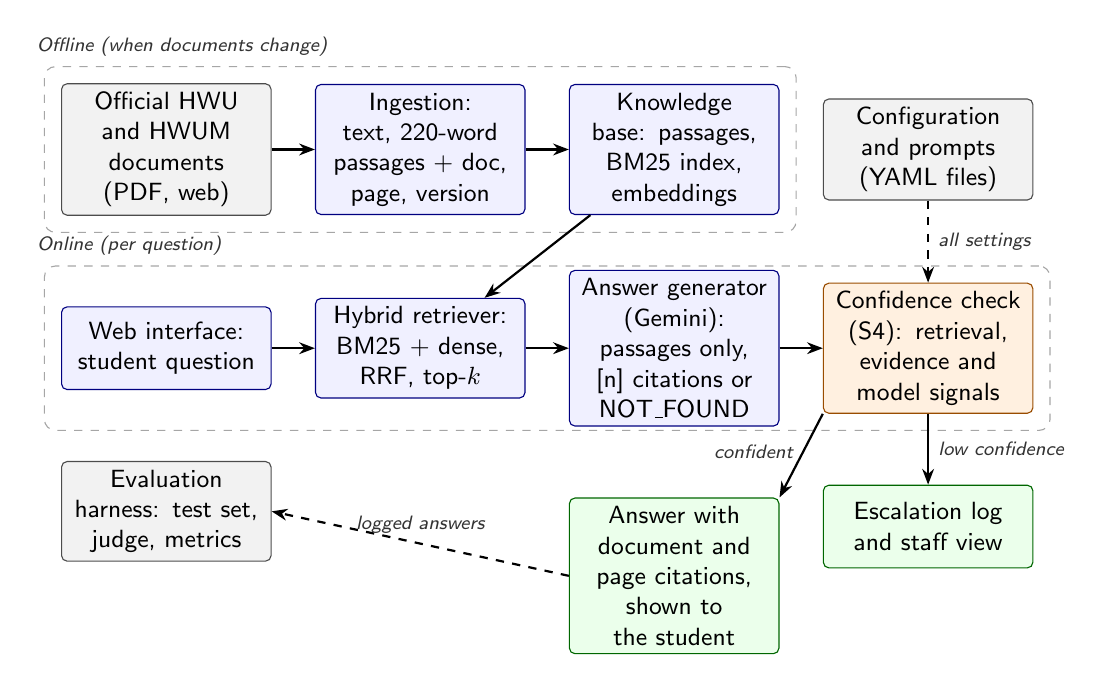
\begin{tikzpicture}[font=\sffamily\small, node distance=0.55cm and 0.55cm,
  box/.style={draw=blue!50!black,fill=blue!6,rounded corners=2pt,align=center,minimum height=1.05cm,text width=2.45cm,inner sep=3pt},
  s4/.style={box,fill=orange!12,draw=orange!60!black},
  outb/.style={box,fill=green!8,draw=green!40!black},
  ext/.style={box,fill=gray!10,draw=gray!60!black},
  arr/.style={-{Stealth[length=2mm]},thick},
  grp/.style={draw=gray!70,dashed,rounded corners,inner sep=6pt},
  capt/.style={font=\sffamily\scriptsize\itshape,text=gray!40!black}]
  % offline
  \node[ext] (docs) {Official HWU and HWUM documents (PDF, web)};
  \node[box,right=of docs] (ing) {Ingestion: text, 220-word passages + doc, page, version};
  \node[box,right=of ing] (kb) {Knowledge base: passages, BM25 index, embeddings};
  % online
  \node[box,below=1.15cm of docs] (ui) {Web interface: student question};
  \node[box,right=of ui] (ret) {Hybrid retriever: BM25 + dense, RRF, top-$k$};
  \node[box,right=of ret] (gen) {Answer generator (Gemini): passages only, [n] citations or NOT\_FOUND};
  \node[s4,right=of gen] (conf) {Confidence check (S4): retrieval, evidence and model signals};
  % outputs
  \node[outb,below=0.9cm of gen] (ans) {Answer with document and page citations, shown to the student};
  \node[outb,below=0.9cm of conf] (esc) {Escalation log and staff view};
  \node[ext,below=0.9cm of ui] (eval) {Evaluation harness: test set, judge, metrics};
  \node[ext,right=of kb] (cfg) {Configuration and prompts (YAML files)};
  \draw[arr] (docs)--(ing); \draw[arr] (ing)--(kb);
  \draw[arr] (kb)--(ret);
  \draw[arr] (ui)--(ret); \draw[arr] (ret)--(gen); \draw[arr] (gen)--(conf);
  \draw[arr] (conf.south west)--node[capt,left,pos=0.45]{confident}(ans.north east);
  \draw[arr] (conf)--node[capt,right]{low confidence}(esc);
  \draw[arr,dashed] (ans.west)--node[capt,above]{logged answers}(eval.east);
\draw[arr,dashed] (cfg)--node[capt,right]{all settings}(conf);
  \begin{scope}[on background layer]
    \node[grp,fit=(docs)(kb),label={[capt]above left:Offline (when documents change)}] {};
    \node[grp,fit=(ui)(conf),label={[capt,anchor=south west,xshift=-6pt]north west:Online (per question)}] {};
  \end{scope}
\end{tikzpicture}
}
\caption{System architecture. S3 stops after the answer generator, S2 skips retrieval, and S1 replaces retrieval and generation with FAQ matching.}
\label{fig:arch}
\end{figure}

\subsubsection{Use Cases} \label{sec:design_usecase}

Figure~\ref{fig:usecase} shows the use cases. A \emph{student} asks a question, reads the answer and its sources, and is referred to Student Services when the evidence is too weak. \emph{Staff} view and resolve escalated questions, and the \emph{maintainer} updates the documents, configures the system and runs the evaluation.

\begin{figure}[H]
\centering
\resizebox{0.66\linewidth}{!}{% Use case diagram (Figure: use cases). TikZ, so it can be edited in Overleaf.
% Needs \usepackage{tikz} with the arrows.meta, positioning, fit, backgrounds and shapes.geometric libraries.
\begin{tikzpicture}[font=\sffamily\small,
  uc/.style={ellipse,draw=blue!50!black,fill=blue!6,minimum width=3.6cm,minimum height=0.95cm,align=center,inner sep=1pt},
  dep/.style={-{Stealth[length=2mm]},dashed},
  lab/.style={font=\sffamily\scriptsize,fill=white,inner sep=1pt}]
  % stick figure: \actor{name}{x,y}{label}
  \newcommand{\actor}[3]{%
    \begin{scope}[shift={(#2)}]
      \draw (0,0.55) circle (0.17); \draw (0,0.38)--(0,-0.1); \draw (-0.3,0.22)--(0.3,0.22);
      \draw (0,-0.1)--(-0.22,-0.5); \draw (0,-0.1)--(0.22,-0.5);
      \node[align=center,below] at (0,-0.5) {#3};
      \coordinate (#1) at (0,0.1);
    \end{scope}}
  \draw[rounded corners,gray] (1.6,-5.65) rectangle (11.4,2.95);
  \node[font=\sffamily\bfseries] at (6.45,2.65) {Student Support Assistant};
  % student side
  \node[uc] (ask) at (4,1.6) {Ask a question};
  \node[uc] (view) at (4,-1.5) {View answer\\with citations};
  \node[uc] (open) at (4,-3.6) {Open cited\\document page};
  \node[uc] (ref) at (4,0.0) {Be referred to\\Student Services};
  % system and staff side
  \node[uc] (gen) at (9.0,1.6) {Retrieve passages and\\generate answer};
  \node[uc] (esc) at (9.0,0.1) {View escalated\\questions};
  \node[uc] (res) at (9.0,-1.5) {Resolve an\\escalation};
  \node[uc] (upd) at (9.0,-2.75) {Update document\\snapshot};
  \node[uc] (cfg) at (9.0,-3.85) {Configure system\\and thresholds};
  \node[uc] (run) at (9.0,-4.95) {Run evaluation};
  \actor{stu}{0,-0.5}{Student}
  \actor{llm}{13,1.4}{Gemini API\\(external)}
  \actor{stf}{13,-0.9}{Student Services\\staff}
  \actor{mnt}{13,-4.0}{Maintainer\\(developer)}
  \draw (stu)--(ask.west); \draw (stu)--(view.west); \draw (stu)--(ref.west);
  \draw (gen.east)--(llm);
  \draw (esc.east)--(stf); \draw (res.east)--(stf);
  \draw (upd.east)--(mnt); \draw (cfg.east)--(mnt); \draw (run.east)--(mnt);
  \draw[dep] (ask)--node[lab]{\guillemotleft include\guillemotright}(gen);
  \draw[dep] (open)--node[lab]{\guillemotleft extend\guillemotright}(view);
  \draw[dep] (ref)--node[lab]{\guillemotleft extend\guillemotright\ (weak evidence)}(ask);
  \draw[dep] (res)--node[lab]{\guillemotleft include\guillemotright}(esc);
\end{tikzpicture}
}
\caption{Use case diagram.}
\label{fig:usecase}
\end{figure}

\subsubsection{User Interface} \label{sec:design_ui}

A working prototype of the interface, called AskWatt, was built with Streamlit and connected to S3 (Figure~\ref{fig:ui}). Citation numbers look like highlighter marks, and each source shows its page number with a link that opens that page of the official PDF, so students can check the answer themselves. When the documents do not cover a question, the student is told so and given an escalation reference instead of a dead end, and staff see these questions in a separate view. The interface asks students not to type personal details (NF1) and stores only the question text.

\begin{figure}[H]
\centering
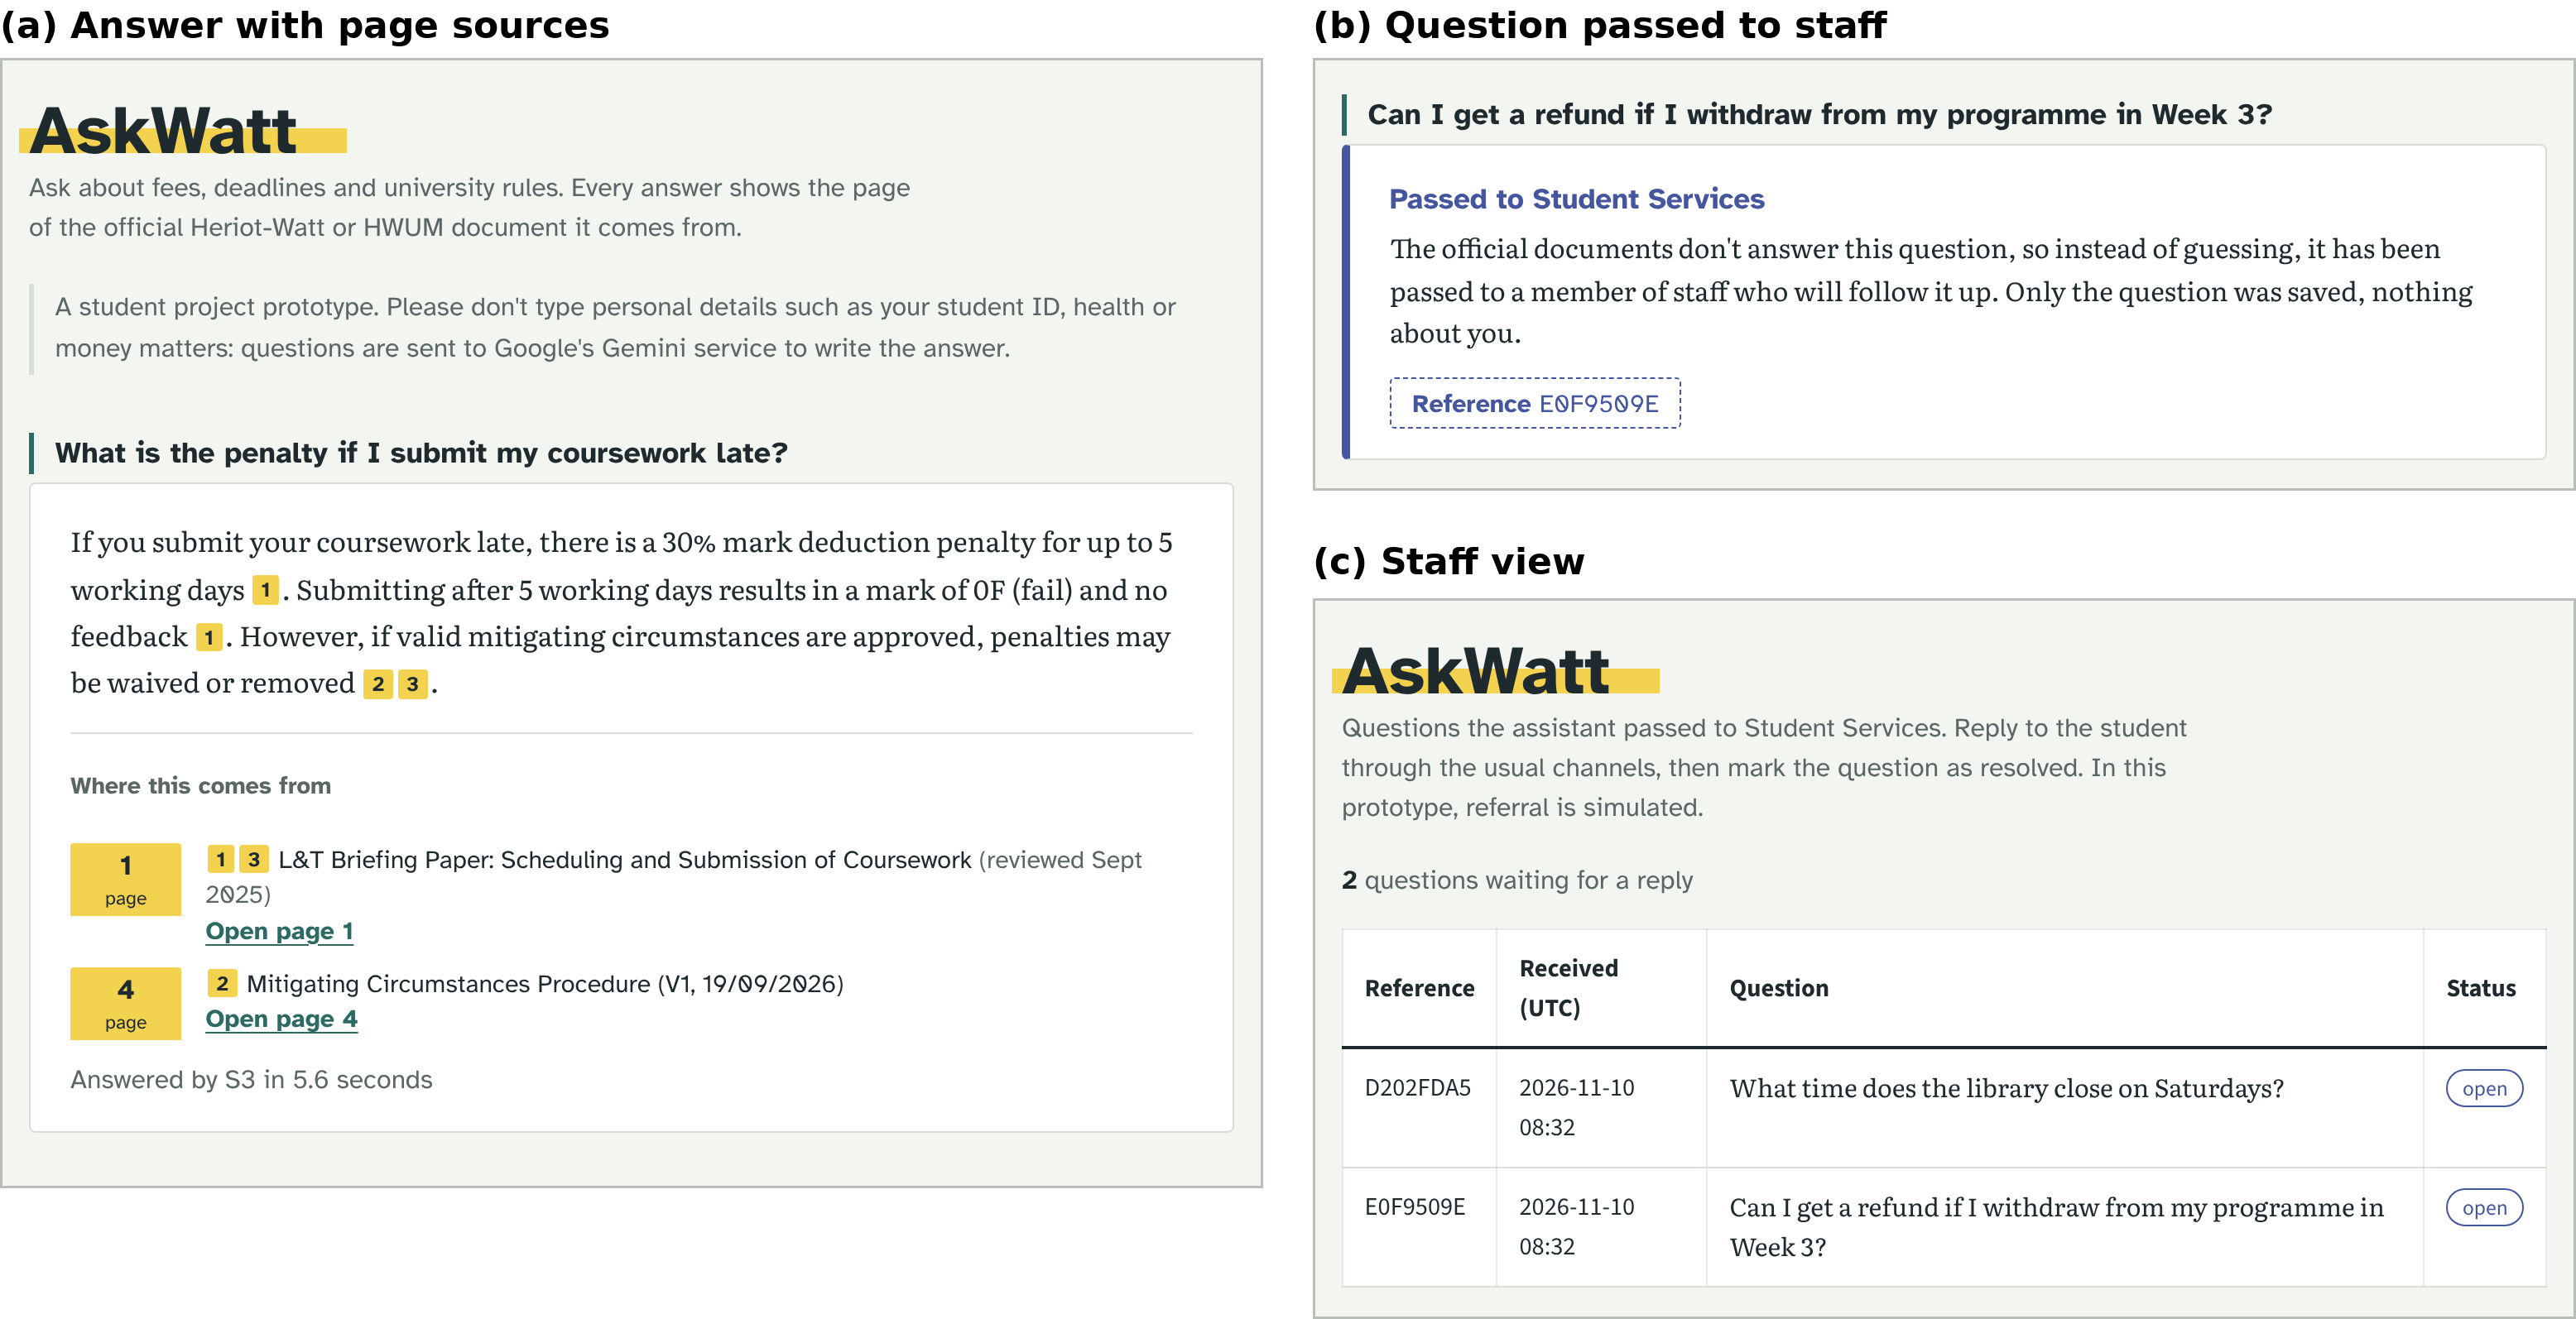
\includegraphics[width=\linewidth]{images/ui_prototype.png}
\caption{The AskWatt prototype connected to S3: (a) an answer with page-level sources, (b) a question the documents do not cover, passed to Student Services, and (c) the staff view of passed questions.}
\label{fig:ui}
\end{figure}

\subsection{Evaluation Plan} \label{sec:method_eval}

\textbf{Test set.} About 200 questions written from the documents, including paraphrases, questions affected by outdated document versions, and about 40 that the documents cannot answer, written using the categories of \citet{peng2025unanswerability}. Each answerable question has a gold answer and supporting quote. About 60 questions are used for all tuning (development set) and the other 140 only once, for the final results (test set).

\textbf{Experiments and metrics.} E1 compares S1, S2 and S3 (RQ1); E2 changes one retrieval choice at a time in S3 (RQ2); E3 compares the confidence signals and thresholds of S4 (RQ3); and E4, approved by ethics in November 2026, asks 10 to 15 HWUM students in Semester 2 Weeks 6 to 8, once S4 is in the interface, to try it and complete the System Usability Scale (SUS) \cite{brooke1996sus} and trust items (RQ4). The main measures are correctness, faithfulness, citation accuracy, retrieval hit rate, the share of wrong and wrongly escalated answers, latency and cost. Answers are labelled by hand on the development set and by an LLM judge on the rest, but only if the judge agrees with my labels (Cohen's $\kappa \geq 0.6$).

\textbf{Analysis.} Because all systems answer the same questions, comparisons use paired tests (McNemar's test for correct and wrong answers), with Holm's correction for the several comparisons in each experiment and bootstrap confidence intervals \cite{dror2018hitchhiker}. Every failure is given a category, such as a retrieval miss, an unsupported claim or a missed escalation, so the results explain why systems fail, not only how often.

\subsection{Success Criteria} \label{sec:method_success}

The criteria were set from the pilot and the literature and are measured on the test set:
\begin{description}
  \item[SC1] S3 is correct on at least 80\% of answerable test questions, at least 20 percentage points more than S2, and significantly more often correct than S1 and S2 (McNemar, Holm-corrected $p < 0.05$). Significance alone is easy with 140 questions, so the target and gap carry the claim; 80\% allows for a harder set than the pilot and is below the 90\% reported for an admissions RAG system \cite{chen2024admission}.
  \item[SC2] At least 85\% of S3's citations support the answer; open-domain systems reach about half \cite{liu2023verifiability}, and a small, closed knowledge base should do better.
  \item[SC3] S4 at least halves the share of wrong answers compared with S3 while wrongly escalating no more than 20\% of answerable questions, since a wrong answer about a fee or penalty costs a student more than a short wait for staff.
  \item[SC4] The best search setting finds the right passage in the top five for at least 90\% of answerable questions.
  \item[SC5] The median response time is 10 seconds or less and the total API cost is below RM100.
  \item[SC6] In E4, the mean SUS score is at least 68, at least matching the 67.75 reported for BarkPlug \cite{neupane2024barkplug}.
\end{description}

% Feasibility
%%%%%%%%%%%%%%%%%%%%
\section{Feasibility} \label{cha:feas}

The project rests on four assumptions: the official documents can be collected and cited at page level; retrieval finds the right passages; grounded generation answers correctly, cites and declines within the cost and time limits; and a cheap signal can separate answerable from unanswerable questions. Preliminary work in Weeks 4 to 9 tested each one with a pilot of 32 questions written from five documents: 26 that follow the documents' wording (20 answerable, 6 unanswerable) and 6 added later to test paraphrases and near-misses (4 answerable, 2 unanswerable). With so few questions, all pilot numbers are indicative, not final results.

\subsection{Document Sources and Ingestion} \label{sec:feas_docs}

An audit in Weeks 4 and 5 found 27 sources. The 23 official ones come from at least five university offices: 12 apply to all Heriot-Watt campuses, 9 only to Malaysia and 2 to one School or a mix; 6 of the 23 are outdated versions still online (4 university-wide, 2 Malaysian), kept for staleness tests. They cover fees and payment (7), mitigating circumstances (5), assessment and progression (5), coursework deadlines and late submission (3), academic regulations (2) and financial aid (1). Three agent websites and another university's page were excluded as unofficial. Five PDFs were ingested into 45 passages tagged with document and page. Checking the gold answers showed that text extraction had misread a fee table; rendering the page gave the correct fee (RM24,200 per semester), so tables will be checked visually before the test set is fixed.

\subsection{Pilot Study} \label{sec:feas_pilot}

\textbf{Retrieval.} Table~\ref{tab:pilot_ret} compares the five retrievers on the 24 answerable questions. Hybrid retrieval was best (hit@1 0.71, MRR 0.78) and tied with stemmed BM25 on hit@5 (0.92). The lexical and dense methods failed on different questions (dense search missed three gold passages that BM25 found, and BM25 missed two that dense search found), so combining them helped, consistent with BEIR \cite{thakur2021beir}. Stemming raised BM25's MRR from 0.68 to 0.72. S3 therefore uses hybrid retrieval with five passages.

\begin{table}[tbp]
\caption{Retrieval pilot on 24 answerable questions (top five passages).}
\label{tab:pilot_ret}
\footnotesize
\begin{tabular}{lccc}
\toprule
Method & Hit@1 & Hit@5 & MRR \\
\midrule
TF-IDF & 0.46 & 0.83 & 0.61 \\
BM25 & 0.58 & 0.88 & 0.68 \\
BM25 with stemming & 0.58 & \textbf{0.92} & 0.72 \\
Dense (bge-small) & 0.62 & 0.83 & 0.72 \\
\textbf{Hybrid (RRF)} & \textbf{0.71} & \textbf{0.92} & \textbf{0.78} \\
\bottomrule
\end{tabular}
\end{table}

\textbf{Systems.} Table~\ref{tab:pilot_sys} compares S1 to S3. S3 answered all 24 answerable questions correctly, including the four paraphrases, cited a source every time (20 of 24 on the gold page) and declined all 8 unanswerable questions, including both near-misses. S2 was fully correct on only 8 and answered 6 of the 8 questions it should have declined, for example inventing a monthly late-payment charge and an appeal deadline that no document contains: the hallucination problem of Section~\ref{sec:back_halluc}. S1 returned the wrong FAQ answer confidently when a question shared its words (10 wrong), yet declined 6 of the 8 unanswerable questions, echoing Walert's finding that a simpler system declines more readily than an LLM \cite{cherumanal2024walert}. Five of the 64 LLM answers were cut off because Gemini's hidden reasoning tokens count towards the 1,024-token output limit, which will be raised before the evaluation. The reference labels were drafted with AI assistance, checked against each gold answer and its exact source quote with deterministic number matching (evidence file in the repository) and reviewed by me. An LLM judge agreed with them on 90 of 96 answers ($\kappa = 0.91$; all six disagreements are one-grade differences on S2, which I decided), and will be validated again against my own hand labels on the development set. S3's perfect score is a ceiling effect, not proof that it is error-free: even the paraphrases needed only one passage, so the test set adds outdated versions, two-passage questions and the unanswerable categories of \citet{peng2025unanswerability}.

\begin{table}[tbp]
\caption{Pilot results for S1--S3 on 24 answerable and 8 unanswerable questions, including six paraphrased or near-miss questions (indicative only).}
\label{tab:pilot_sys}
\footnotesize
\begin{tabular}{lcccccc}
\toprule
& \multicolumn{4}{c}{Answerable (of 24)} & Unanswerable & Median \\
\cmidrule(lr){2-5}
System & Correct & Partial & Wrong & Escalated & declined (of 8) & latency (s) \\
\midrule
S1 FAQ & 8 & 1 & 10 & 5 & 6 & 0.00 \\
S2 Plain LLM & 8 & 6 & 7 & 3 & 2 & 3.81 \\
S3 RAG & \textbf{24} & 0 & 0 & 0 & \textbf{8} & 3.12 \\
\bottomrule
\end{tabular}
\end{table}

\textbf{Escalation signals.} Figure~\ref{fig:signals} shows two candidate S4 signals (AUROC with bootstrap 95\% intervals). The top dense score separated the groups fairly well (0.85 [0.69, 0.97]); the top BM25 score (0.71 [0.52, 0.88]) and the score gaps (0.55 to 0.58) did worse. Near-misses explain why: the late-payment and appeal questions outscored eight and ten answerable questions, because the documents are on topic but lack the answer. The model signal, one extra Gemini call asking whether the passages are enough, scored every answerable question 80 to 100 and every unanswerable one 0. This is weak evidence: there are eight negatives, the same model writes S3's answers and S3 had already declined all eight, so E3 must show that the signal adds to S3's own NOT\_FOUND.

\begin{figure}[tbp]
\centering
\resizebox{\linewidth}{!}{% S4 signal plot (Figure: signals). Generated by eval/plot_signals.py from eval/results/confidence_pilot.csv;
% do not edit by hand. Needs \usepackage{tikz}.
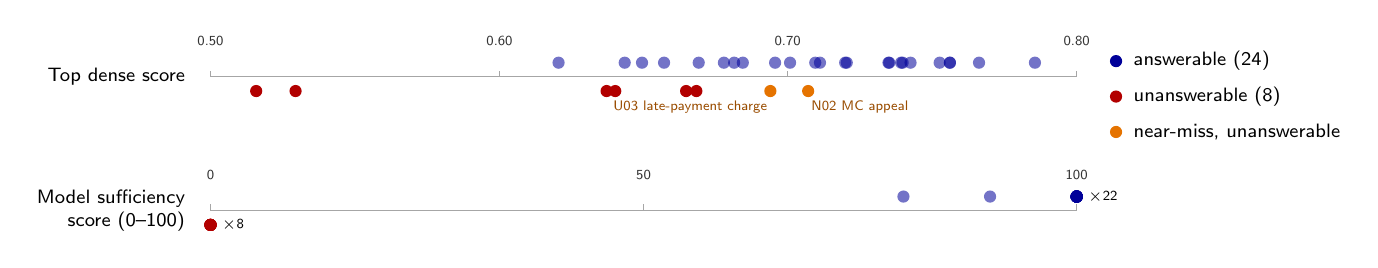
\begin{tikzpicture}[font=\sffamily\small]
  \node[anchor=east,font=\sffamily\scriptsize,align=right] at (-0.2,1.70) {Top dense score};
  \draw[gray!70] (0,1.70) -- (11.0,1.70);
  \draw[gray!70] (0.00,1.70) -- (0.00,1.78);
  \node[font=\sffamily\tiny,text=gray!40!black] at (0.00,2.15) {0.50};
  \draw[gray!70] (3.67,1.70) -- (3.67,1.78);
  \node[font=\sffamily\tiny,text=gray!40!black] at (3.67,2.15) {0.60};
  \draw[gray!70] (7.33,1.70) -- (7.33,1.78);
  \node[font=\sffamily\tiny,text=gray!40!black] at (7.33,2.15) {0.70};
  \draw[gray!70] (11.00,1.70) -- (11.00,1.78);
  \node[font=\sffamily\tiny,text=gray!40!black] at (11.00,2.15) {0.80};
  \fill[blue!60!black,opacity=0.55] (9.76,1.88) circle (2.2pt);
  \fill[blue!60!black,opacity=0.55] (8.77,1.88) circle (2.2pt);
  \fill[blue!60!black,opacity=0.55] (5.26,1.88) circle (2.2pt);
  \fill[blue!60!black,opacity=0.55] (8.62,1.88) circle (2.2pt);
  \fill[blue!60!black,opacity=0.55] (6.20,1.88) circle (2.2pt);
  \fill[blue!60!black,opacity=0.55] (9.26,1.88) circle (2.2pt);
  \fill[blue!60!black,opacity=0.55] (8.06,1.88) circle (2.2pt);
  \fill[blue!60!black,opacity=0.55] (10.47,1.88) circle (2.2pt);
  \fill[blue!60!black,opacity=0.55] (7.74,1.88) circle (2.2pt);
  \fill[blue!60!black,opacity=0.55] (5.48,1.88) circle (2.2pt);
  \fill[blue!60!black,opacity=0.55] (4.42,1.88) circle (2.2pt);
  \fill[blue!60!black,opacity=0.55] (6.76,1.88) circle (2.2pt);
  \fill[blue!60!black,opacity=0.55] (8.08,1.88) circle (2.2pt);
  \fill[blue!60!black,opacity=0.55] (8.79,1.88) circle (2.2pt);
  \fill[blue!60!black,opacity=0.55] (7.68,1.88) circle (2.2pt);
  \fill[blue!60!black,opacity=0.55] (9.39,1.88) circle (2.2pt);
  \fill[blue!60!black,opacity=0.55] (8.89,1.88) circle (2.2pt);
  \fill[blue!60!black,opacity=0.55] (9.39,1.88) circle (2.2pt);
  \fill[blue!60!black,opacity=0.55] (8.61,1.88) circle (2.2pt);
  \fill[blue!60!black,opacity=0.55] (5.76,1.88) circle (2.2pt);
  \fill[red!70!black] (0.58,1.52) circle (2.2pt);
  \fill[red!70!black] (5.03,1.52) circle (2.2pt);
  \fill[orange!90!black] (7.11,1.52) circle (2.2pt);
  \node[font=\sffamily\tiny,text=orange!60!black,anchor=north east,inner sep=1pt] at (7.11,1.44) {U03 late-payment charge};
  \fill[red!70!black] (6.17,1.52) circle (2.2pt);
  \fill[red!70!black] (1.08,1.52) circle (2.2pt);
  \fill[red!70!black] (6.04,1.52) circle (2.2pt);
  \fill[blue!60!black,opacity=0.55] (6.52,1.88) circle (2.2pt);
  \fill[blue!60!black,opacity=0.55] (7.36,1.88) circle (2.2pt);
  \fill[blue!60!black,opacity=0.55] (7.17,1.88) circle (2.2pt);
  \fill[blue!60!black,opacity=0.55] (6.65,1.88) circle (2.2pt);
  \fill[red!70!black] (5.14,1.52) circle (2.2pt);
  \fill[orange!90!black] (7.59,1.52) circle (2.2pt);
  \node[font=\sffamily\tiny,text=orange!60!black,anchor=north west,inner sep=1pt] at (7.59,1.44) {N02 MC appeal};
  \node[anchor=east,font=\sffamily\scriptsize,align=right] at (-0.2,0.00) {Model sufficiency\\score (0--100)};
  \draw[gray!70] (0,0.00) -- (11.0,0.00);
  \draw[gray!70] (0.00,0.00) -- (0.00,0.08);
  \node[font=\sffamily\tiny,text=gray!40!black] at (0.00,0.45) {0};
  \draw[gray!70] (5.50,0.00) -- (5.50,0.08);
  \node[font=\sffamily\tiny,text=gray!40!black] at (5.50,0.45) {50};
  \draw[gray!70] (11.00,0.00) -- (11.00,0.08);
  \node[font=\sffamily\tiny,text=gray!40!black] at (11.00,0.45) {100};
  \fill[blue!60!black,opacity=0.55] (11.00,0.18) circle (2.2pt);
  \fill[blue!60!black,opacity=0.55] (11.00,0.18) circle (2.2pt);
  \fill[blue!60!black,opacity=0.55] (11.00,0.18) circle (2.2pt);
  \fill[blue!60!black,opacity=0.55] (8.80,0.18) circle (2.2pt);
  \fill[blue!60!black,opacity=0.55] (9.90,0.18) circle (2.2pt);
  \fill[blue!60!black,opacity=0.55] (11.00,0.18) circle (2.2pt);
  \fill[blue!60!black,opacity=0.55] (11.00,0.18) circle (2.2pt);
  \fill[blue!60!black,opacity=0.55] (11.00,0.18) circle (2.2pt);
  \fill[blue!60!black,opacity=0.55] (11.00,0.18) circle (2.2pt);
  \fill[blue!60!black,opacity=0.55] (11.00,0.18) circle (2.2pt);
  \fill[blue!60!black,opacity=0.55] (11.00,0.18) circle (2.2pt);
  \fill[blue!60!black,opacity=0.55] (11.00,0.18) circle (2.2pt);
  \fill[blue!60!black,opacity=0.55] (11.00,0.18) circle (2.2pt);
  \fill[blue!60!black,opacity=0.55] (11.00,0.18) circle (2.2pt);
  \fill[blue!60!black,opacity=0.55] (11.00,0.18) circle (2.2pt);
  \fill[blue!60!black,opacity=0.55] (11.00,0.18) circle (2.2pt);
  \fill[blue!60!black,opacity=0.55] (11.00,0.18) circle (2.2pt);
  \fill[blue!60!black,opacity=0.55] (11.00,0.18) circle (2.2pt);
  \fill[blue!60!black,opacity=0.55] (11.00,0.18) circle (2.2pt);
  \fill[blue!60!black,opacity=0.55] (11.00,0.18) circle (2.2pt);
  \fill[red!70!black] (0.00,-0.18) circle (2.2pt);
  \fill[red!70!black] (0.00,-0.18) circle (2.2pt);
  \fill[red!70!black] (0.00,-0.18) circle (2.2pt);
  \fill[red!70!black] (0.00,-0.18) circle (2.2pt);
  \fill[red!70!black] (0.00,-0.18) circle (2.2pt);
  \fill[red!70!black] (0.00,-0.18) circle (2.2pt);
  \fill[blue!60!black,opacity=0.55] (11.00,0.18) circle (2.2pt);
  \fill[blue!60!black,opacity=0.55] (11.00,0.18) circle (2.2pt);
  \fill[blue!60!black,opacity=0.55] (11.00,0.18) circle (2.2pt);
  \fill[blue!60!black,opacity=0.55] (11.00,0.18) circle (2.2pt);
  \fill[red!70!black] (0.00,-0.18) circle (2.2pt);
  \fill[red!70!black] (0.00,-0.18) circle (2.2pt);
  \node[font=\sffamily\tiny,anchor=west,inner sep=1pt] at (11.10,0.18) {$\times$22};
  \node[font=\sffamily\tiny,anchor=west,inner sep=1pt] at (0.10,-0.18) {$\times$8};
  \fill[blue!60!black] (11.50,1.90) circle (2.2pt);
  \node[right,font=\sffamily\scriptsize] at (11.60,1.90) {answerable (24)};
  \fill[red!70!black] (11.50,1.45) circle (2.2pt);
  \node[right,font=\sffamily\scriptsize] at (11.60,1.45) {unanswerable (8)};
  \fill[orange!90!black] (11.50,1.00) circle (2.2pt);
  \node[right,font=\sffamily\scriptsize] at (11.60,1.00) {near-miss, unanswerable};
\end{tikzpicture}
}
\caption{Two S4 signals for the 32 pilot questions: answerable above each line, unanswerable below; near-misses are labelled.}
\label{fig:signals}
\end{figure}

\subsection{Cost, Latency and Prototype} \label{sec:feas_proto}

The whole pilot, including the judge and the model signal, used 192 API calls and cost US\$0.37. S3 cost US\$0.0034 per question with a median latency of 3.1 seconds, well within NF4. Projected from these measured costs, the evaluation would cost about US\$5.80 (RM26 at a cautious RM4.50 per US dollar): E1 US\$1.21, E2 US\$2.44 (twelve configurations on the 60 development questions; retrieval-only metrics need no LLM call), E3 US\$0.43 and judging US\$1.69, far below NF5's RM100 even with reruns. The interface (Section~\ref{sec:design_ui}) already runs the pipeline end to end on a laptop, and twelve unit tests pass.

In summary, early evidence supports the first three assumptions and no blocking problem was found. The fourth is only partly supported: retrieval scores miss near-misses, and the model signal, although it separated every pilot question, rests on eight unanswerable questions. The main remaining risks are these near-misses and the time needed to write 200 questions; they are addressed by writing near-misses into the development set, comparing three signal groups for S4 and building the test set first (Section~\ref{sec:method_plan}).

% Conclusions
%%%%%%%%%%%%%%%%%%%%
\section{Conclusions} \label{cha:concl}

HWUM students need quick, correct answers to questions about fees, deadlines and regulations, but the official information is spread across many documents, and general chatbots answer such questions confidently and often wrongly. The literature shows that retrieval-augmented generation can ground answers in documents, but that citations, abstention and escalation must be measured rather than assumed, and that existing university chatbots rarely test questions they cannot answer. This project will therefore compare an FAQ baseline, a plain LLM, RAG with citations and RAG with confidence-based escalation on the same HWUM documents and test set, using paired statistics and error analysis. The feasibility work shows that the documents, retrieval, grounded generation and a working interface are in place at low cost, and that candidate escalation signals exist but need a larger, harder test set before they can be trusted. Semester 2 therefore concentrates on the test set, the confidence check, the evaluation and the approved usability study.


%%%%%%%%%%%%%%%%%%%%%%%%%%%%%%%%%%%%%%%%%%%%%%%%%%
% BACK MATTER
%%%%%%%%%%%%%%%%%%%%%%%%%%%%%%%%%%%%%%%%%%%%%%%%%%

% References
% list of references

\newpage
\renewcommand{\bibname}{References} % change name to References
% \phantomsection
% \addcontentsline{toc}{section}{References}
\bibliography{references}
% \bibliographystyle{plainnat}

% using Harvard style
% \bibliographystyle{agsm}

% using ACM style (defined in acm_settings.tex)
\bibliographystyle{ACM-Reference-Format}

% using APA style (requires apacite package)
% \bibliographystyle{apacite}

% Appendices
\newpage
\appendix

\crefalias{chapter}{appendixchapter} % for appendix crossreferences

\section{Project Management}

\subsection{Gantt Chart} \label{sec:app_gantt}

Figure~\ref{fig:gantt1} shows the activities carried out in Semester 1 and Figure~\ref{fig:gantt2} the plan for Semester 2. Weeks are teaching weeks: Semester 1 Week 1 began on 14 September 2026 and Semester 2 Week 1 begins on 18 January 2027. Diamonds are milestones and arrows show dependencies. No project work is planned during the December exams, and Weeks 9 and 10 of Semester 2 have no experiments scheduled, so they act as a buffer. Tasks are tracked weekly on a Notion board (\url{https://app.notion.com/p/6f58a0a5b3c549b98d6a51e9b8e36ae7}) and all code, results and records are in a GitHub repository (\url{https://github.com/sutin1215/grounded-university-support-assistant}); both are shared with the supervisor.

\begin{figure}[h]
\centering
\resizebox{\linewidth}{!}{%
\begin{ganttchart}[hgrid, vgrid={*{1}{dotted}}, x unit=0.62cm, y unit chart=0.5cm, y unit title=0.55cm,
  title label font=\scriptsize, bar label font=\footnotesize, milestone label font=\footnotesize\itshape,
  bar/.append style={fill=blue!25}, milestone/.append style={fill=orange!80}]{1}{12}
\gantttitle{Semester 1, 2026 (teaching weeks)}{12} \\
\gantttitlelist{1,...,12}{1} \\
\ganttbar{Topic, supervision and records}{1}{3} \\
\ganttbar{Literature review}{2}{9} \\
\ganttbar{Document audit and source list}{4}{5} \\
\ganttbar{Ethics application}{4}{7} \\
\ganttbar{Pilot: ingestion, retrieval, S1}{7}{7} \\
\ganttbar{Pilot: S2, S3, judge, S4 signals}{7}{8} \\
\ganttbar{Interface prototype}{8}{8} \\
\ganttbar{D1 report}{6}{11} \\
\ganttbar{D2 video}{10}{11} \\
\ganttmilestone{Ethics application submitted (26 Oct)}{7} \\
\ganttmilestone{D1 and D2 submitted (26 Nov)}{11}
\end{ganttchart}}
\caption{Semester 1: activities carried out in Weeks 1 to 11. Week 6 was a study week.}
\label{fig:gantt1}
\end{figure}

\begin{figure}[h]
\centering
\resizebox{\linewidth}{!}{%
\begin{ganttchart}[hgrid, vgrid={*{1}{dotted}}, x unit=0.62cm, y unit chart=0.5cm, y unit title=0.55cm,
  title label font=\scriptsize, bar label font=\footnotesize, milestone label font=\footnotesize\itshape,
  bar/.append style={fill=blue!25}, milestone/.append style={fill=orange!80},
  link/.style={-{Stealth[length=1.6mm]}, gray, thick}]{1}{16}
\gantttitle{Break}{2} \gantttitle{Semester 2, 2027 (teaching weeks)}{14} \\
\gantttitle{Dec}{1} \gantttitle{Jan}{1} \gantttitlelist{1,...,14}{1} \\
\ganttbar[name=kb]{Knowledge base, 60 dev. questions (after exams)}{1}{2} \\
\ganttbar[name=ts]{Write and label 140 test questions}{3}{5} \\
\ganttbar[name=e2]{E2 retrieval (development set)}{5}{6} \\
\ganttbar[name=s4]{Build and tune S4 (E3)}{6}{7} \\
\ganttbar[name=ui]{Complete interface with S4}{6}{8} \\
\ganttbar[name=fin]{Final test run (E1--E3)}{7}{8} \\
\ganttbar[name=e4]{Usability study E4 (ethics approved)}{8}{10} \\
\ganttbar[name=an]{Analysis and error analysis}{8}{10} \\
\ganttbar[name=d3]{Write dissertation (D3)}{7}{13} \\
\ganttbar[bar/.append style={fill=gray!20}]{Buffer (no experiments)}{11}{12} \\
\ganttmilestone{D3 due (1 Apr)}{13} \\
\ganttbar[bar/.append style={fill=green!25}]{Q\&A session (D5)}{13}{16}
\ganttlink{kb}{ts} \ganttlink{ts}{e2} \ganttlink{e2}{s4} \ganttlink{s4}{fin} \ganttlink{fin}{an} \ganttlink{ui}{e4}
\end{ganttchart}}
\caption{Semester 2 plan. Arrows show dependencies; the usability study needs S4 in the interface.}
\label{fig:gantt2}
\end{figure}

\subsection{Risk Analysis} \label{sec:app_risk}

Table~\ref{tab:risk} rates each risk for likelihood (L) and impact (I) from 1 (very low) to 5 (very high); the score is L$\times$I, where 12 or more is high, 6 to 11 medium and 5 or less low. Each risk has an avoidance step taken in advance and a contingency if it happens anyway. Figure~\ref{fig:heatmap} places the risks on a likelihood--impact grid; the two high risks (R1, R2) are both about time, which is why the plan avoids the exam weeks and keeps Weeks 9--10 free of experiments.

\begin{figure}[H]
\centering
% Risk heat map (Figure: risk heat map). TikZ, so it can be edited in Overleaf.
% Positions must match the L and I columns of the risk register (Table: risk). Colours follow the score
% bands in the text: L x I of 12 or more is high, 6 to 11 medium, 5 or less low.
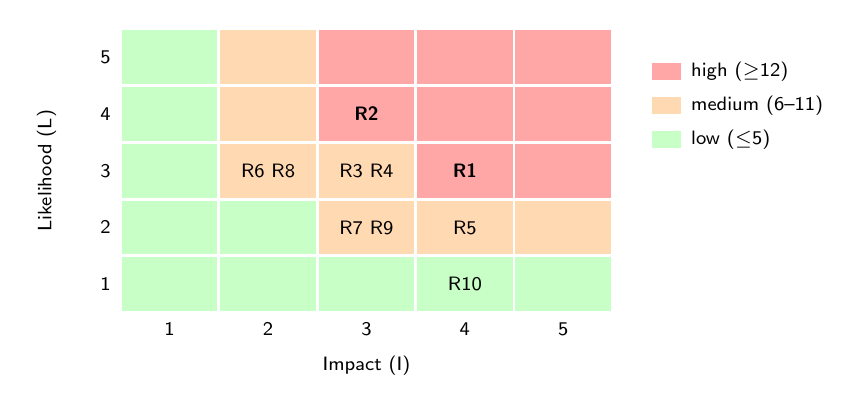
\begin{tikzpicture}[font=\sffamily\scriptsize, x=1.25cm, y=0.72cm]
  % cells, coloured by score band
  \foreach \lik in {1,...,5} {
    \foreach \imp in {1,...,5} {
      \pgfmathtruncatemacro{\score}{\lik*\imp}
      \ifnum\score>11 \def\cellcol{red!35}\else\ifnum\score>5 \def\cellcol{orange!30}\else\def\cellcol{green!22}\fi\fi
      \fill[\cellcol] (\imp-1,\lik-1) rectangle (\imp,\lik);
      \draw[white, line width=1pt] (\imp-1,\lik-1) rectangle (\imp,\lik);
    }
  }
  % axes labels
  \foreach \imp in {1,...,5} \node[below] at (\imp-0.5,0) {\imp};
  \foreach \lik in {1,...,5} \node[left] at (0,\lik-0.5) {\lik};
  \node[below=12pt] at (2.5,0) {Impact (I)};
  \node[rotate=90] at (-0.75,2.5) {Likelihood (L)};
  % risks: (impact, likelihood)
  \node at (3.5,2.5) {\textbf{R1}};          % L3 I4
  \node at (2.5,3.5) {\textbf{R2}};          % L4 I3
  \node at (2.5,2.5) {R3\,\,R4};             % L3 I3
  \node at (3.5,1.5) {R5};                   % L2 I4
  \node at (1.5,2.5) {R6\,\,R8};             % L3 I2
  \node at (2.5,1.5) {R7\,\,R9};             % L2 I3
  \node at (3.5,0.5) {R10};                  % L1 I4
  % legend
  \fill[red!35] (5.4,4.1) rectangle (5.7,4.4); \node[right] at (5.7,4.25) {high ($\geq$12)};
  \fill[orange!30] (5.4,3.5) rectangle (5.7,3.8); \node[right] at (5.7,3.65) {medium (6--11)};
  \fill[green!22] (5.4,2.9) rectangle (5.7,3.2); \node[right] at (5.7,3.05) {low ($\leq$5)};
\end{tikzpicture}

\caption{Risk heat map: each risk placed by its likelihood and impact from Table~\ref{tab:risk}.}
\label{fig:heatmap}
\end{figure}

\begin{table}[H]
\caption{Risk register.}
\label{tab:risk}
\footnotesize
\begin{tabular}{L{0.04\linewidth}L{0.21\linewidth}@{\hspace{4pt}}c@{\hspace{4pt}}c@{\hspace{4pt}}c@{\hspace{6pt}}L{0.25\linewidth}L{0.25\linewidth}}
\toprule
ID & Risk & L & I & Score & Avoidance & Contingency \\
\midrule
R1 & Writing and checking 200 questions takes longer than planned & 3 & 4 & 12 & 60 development questions after the exams; template; about 50 test questions a week in Weeks 1--3 & Reduce to 150 questions, keeping the share of unanswerable ones; report the effect on statistical power \\
R2 & Workload from other courses, including the December exams & 4 & 3 & 12 & No work in exam weeks; weekly sprints; Gantt deadlines; Weeks 9--10 free of experiments & Drop the Could requirement (F7) and shorten E4; keep all Must requirements \\
R3 & S4 signals cannot separate near-miss questions & 3 & 3 & 9 & Put near-miss questions in the development set; compare all three signal groups before fixing the threshold & Report the negative result with the risk--coverage analysis, which still answers RQ3 \\
R4 & Text extraction errors in tables & 3 & 3 & 9 & Check table pages visually; verify every gold quote & Correct the affected passages by hand and record the fix \\
R5 & Gemini model retired, changed or more expensive & 2 & 4 & 8 & Pinned model version; every response cached (NF2); cost far below NF5 & Re-run all LLM systems on another model of the same tier \\
R6 & Too few students take part in the usability study (E4) & 3 & 2 & 6 & Recruit from Week 3 via the approved advert, class channels and the supervisor; short online sessions & Run E4 with those available; report SUS descriptively and state the small sample \\
R7 & LLM judge disagrees with my labels ($\kappa < 0.6$) & 2 & 3 & 6 & Strict grading prompt; validate on the development set & Label all test answers by hand (about 15 hours) \\
R8 & University documents change during the project & 3 & 2 & 6 & Frozen, dated snapshot and source list with access dates & Keep the snapshot; note the change as a limitation \\
R9 & API key exposed through the code repository & 2 & 3 & 6 & Key kept only in an ignored .env file and never committed; repository made private before submission & Revoke and replace the key at once \\
R10 & Laptop failure or data loss & 1 & 4 & 4 & Code on GitHub; documents on OneDrive & Restore from the remote copies; continue on a lab machine \\
\bottomrule
\end{tabular}
\end{table}

\subsection{Professional, Legal, Ethical and Social Issues} \label{sec:app_ples}

\textbf{Professional.} The project follows the BCS Code of Conduct \cite{bcs2022code}. In the public interest, the assistant gives students information from official sources and refers them to staff rather than guessing. Under professional competence and integrity, results are reported honestly: pilot numbers are called indicative, negative results will be reported, and the limits of the system (one LLM family, author-written questions, simulated escalation) are stated. All third-party work, including libraries, models and documents, is acknowledged, and the use of generative AI is declared in Appendix~\ref{sec:app_genai}.

\textbf{Legal.} No personal data is collected or processed by the system, so the Personal Data Protection Act 2010 \cite{pdpa2010} and the UK GDPR that applies to Heriot-Watt as data controller are respected by design: the interface asks students not to type personal details, and only the question text of an escalation is stored. The usability study collects only pseudonymised questionnaire data, handled as described in the approved information sheet. The university documents are protected by copyright \cite{copyright1987}; they are used only for non-commercial research, cited by page rather than copied, and are not redistributed (the PDFs are excluded from the code repository, which is made private before submission). The supervisor confirmed on 13 October 2026 that these public documents may be used. The Gemini API is used under Google's terms for paid services \cite{google2026terms}: prompts and responses are not used to improve Google's products, but Google logs them for a limited period to detect misuse and for legal disclosures, and may store them in any country where it has facilities. Retention, not only training, is therefore a concern, so only public documents and test questions are sent, the interface tells users that questions go to Google's Gemini service and asks them not to type personal details, and the usability study gives participants prepared questions. All software libraries are used under their open-source licences.

\textbf{Ethical.} The main ethical risk is harm from wrong answers about fees, deadlines or penalties. The design reduces it by answering only from official documents, showing sources and escalating when evidence is weak, and the interface tells students that it is a prototype and that official sources and staff decisions take precedence. Sensitive topics such as mental health, personal financial hardship and disciplinary cases are out of scope (Section~\ref{sec:intro_scope}). Students always know they are using an automated system. Ethics approval for the usability study was granted in November 2026; participants give informed consent, can withdraw at any time and are not asked about their own circumstances. Because LLM judges and AI-assisted labelling can be biased, every automatic label is validated against my own labels before it is used.

\textbf{Social.} The assistant is meant to support Student Services, not replace it: it handles routine factual questions and passes everything else to people, so staff can spend more time on cases that need judgement. It could make information more accessible outside office hours, but students who prefer human contact or are less confident in English may benefit less; the English-only scope is stated as a limitation. Over-reliance is reduced by showing sources so students can check answers, and the energy cost of LLM calls is limited by caching and a small knowledge base.


\section{Generative AI Summary} \label{sec:app_genai}

Generative AI was used in two separate ways in this project.

\textbf{As part of the system.} Google's Gemini 3.6 Flash, accessed through its paid API, generates the answers of S2 to S4, gives the S4 model signal and acts as the LLM judge. Only public university documents and test questions are sent to it, never personal data (NF1), and paid-tier prompts are not used to improve Google's products. Its outputs are evaluated rather than trusted: hallucination, citation accuracy and judge agreement are measured (Sections~\ref{sec:method_eval} and~\ref{sec:feas_pilot}).

\textbf{As an assistant while doing the project.} I used Claude (Anthropic), through Claude Code and claude.ai, to: (1) search for related papers and check the bibliographic details of every reference against publisher or repository pages; (2) write and debug code (ingestion, retrieval, the systems, the evaluation scripts and the web interface), which I reviewed, ran and tested; (3) draft the pilot questions, their gold answers and supporting quotes, and the FAQ used by S1, and draft the reference labels for the 96 pilot answers and check them against the source quotes with deterministic matching, after which I reviewed every label and decided the disputed ones (Section~\ref{sec:feas_pilot}); (4) draft and edit parts of this report, including tables and diagrams, from my notes, my supervisor's feedback and the pilot results; and (5) compare the structure of past dissertations with the marking criteria. I reviewed and revised all text and remain responsible for every claim. Every number in this report comes from scripts in the project repository and was checked against their output files, and every reference was checked against its source, to guard against invented references or wrong figures.

\section{Participant Information Sheet and Consent Form} \label{sec:app_forms}

The information sheet and consent form below were submitted with the ethics application on 26 October 2026, which was approved in November 2026. They will be used in the usability study (E4) in Semester 2.

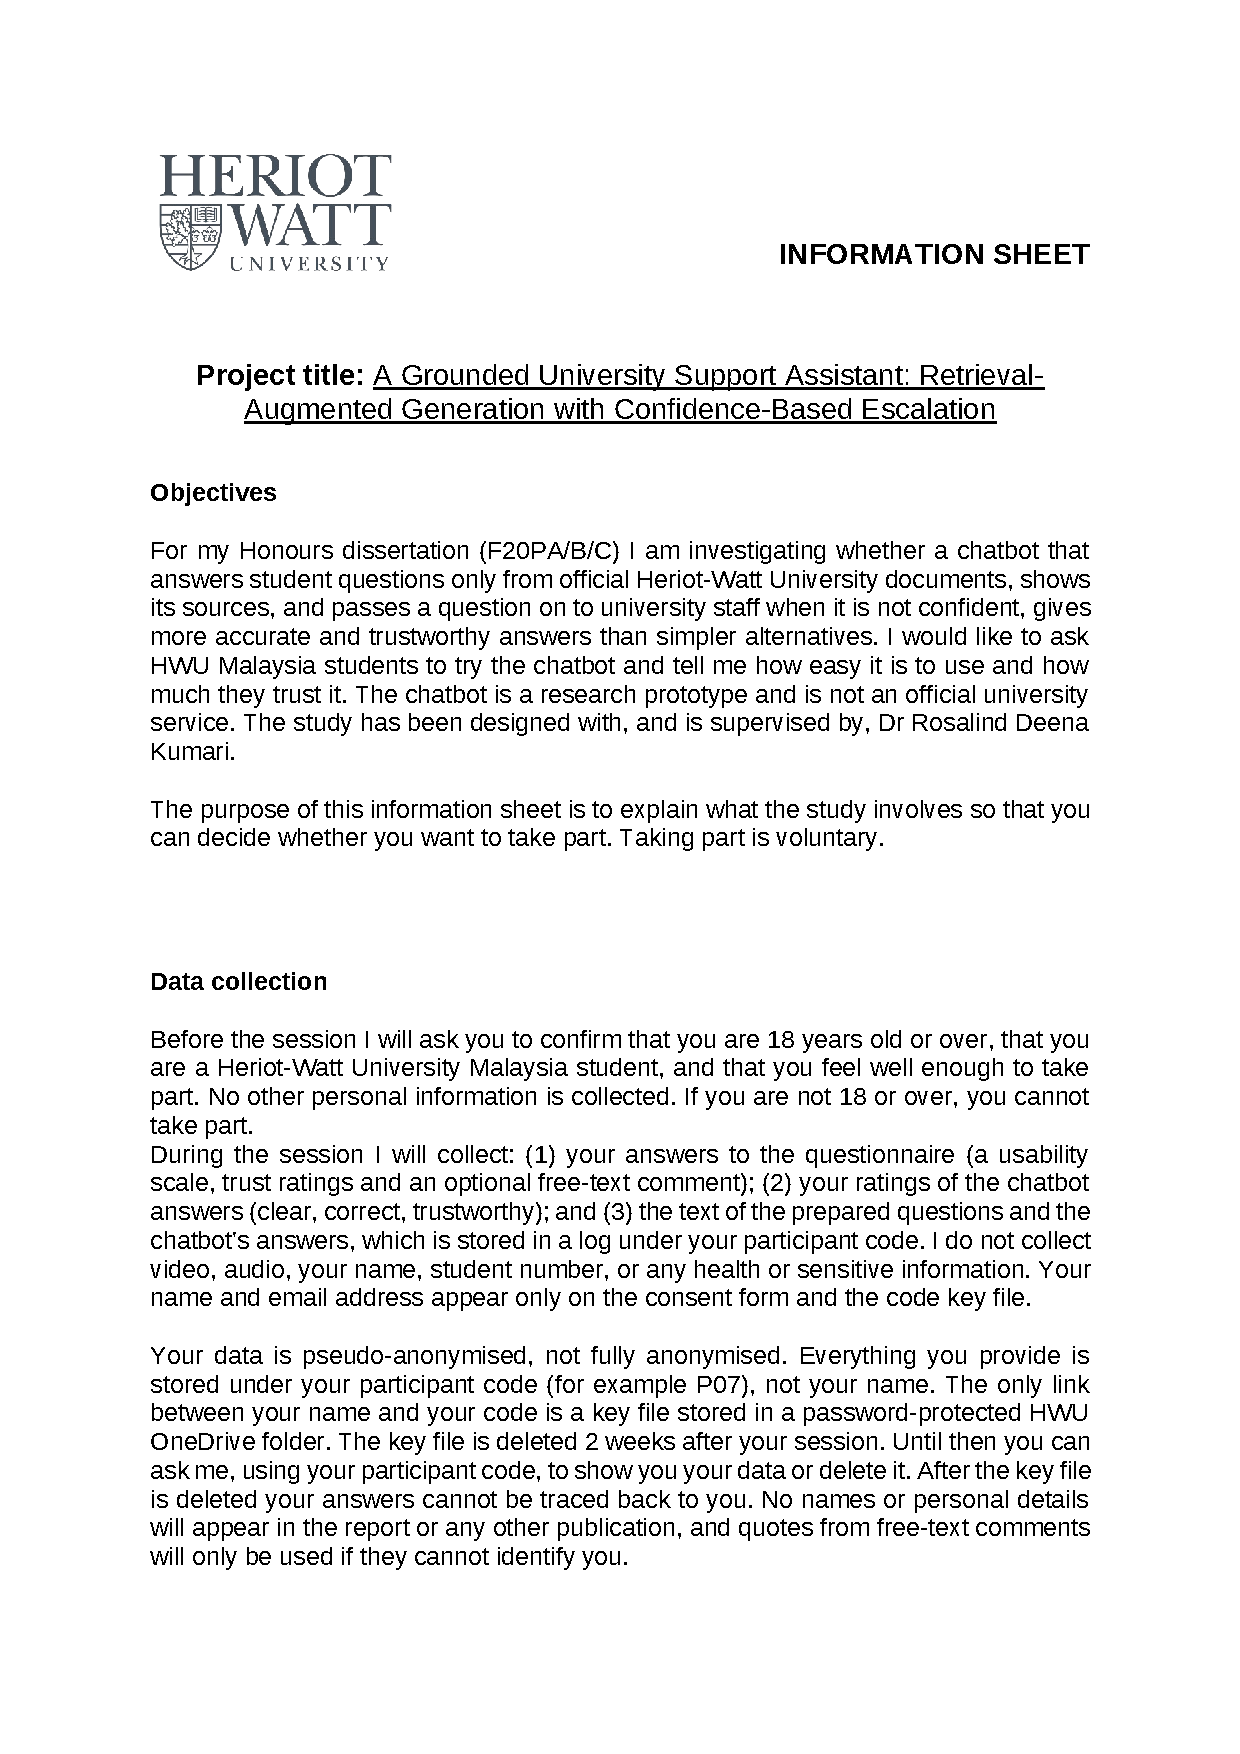
\includepdf[pages=-, scale=0.8, frame, pagecommand={}]{images/appendix_information_sheet.pdf}
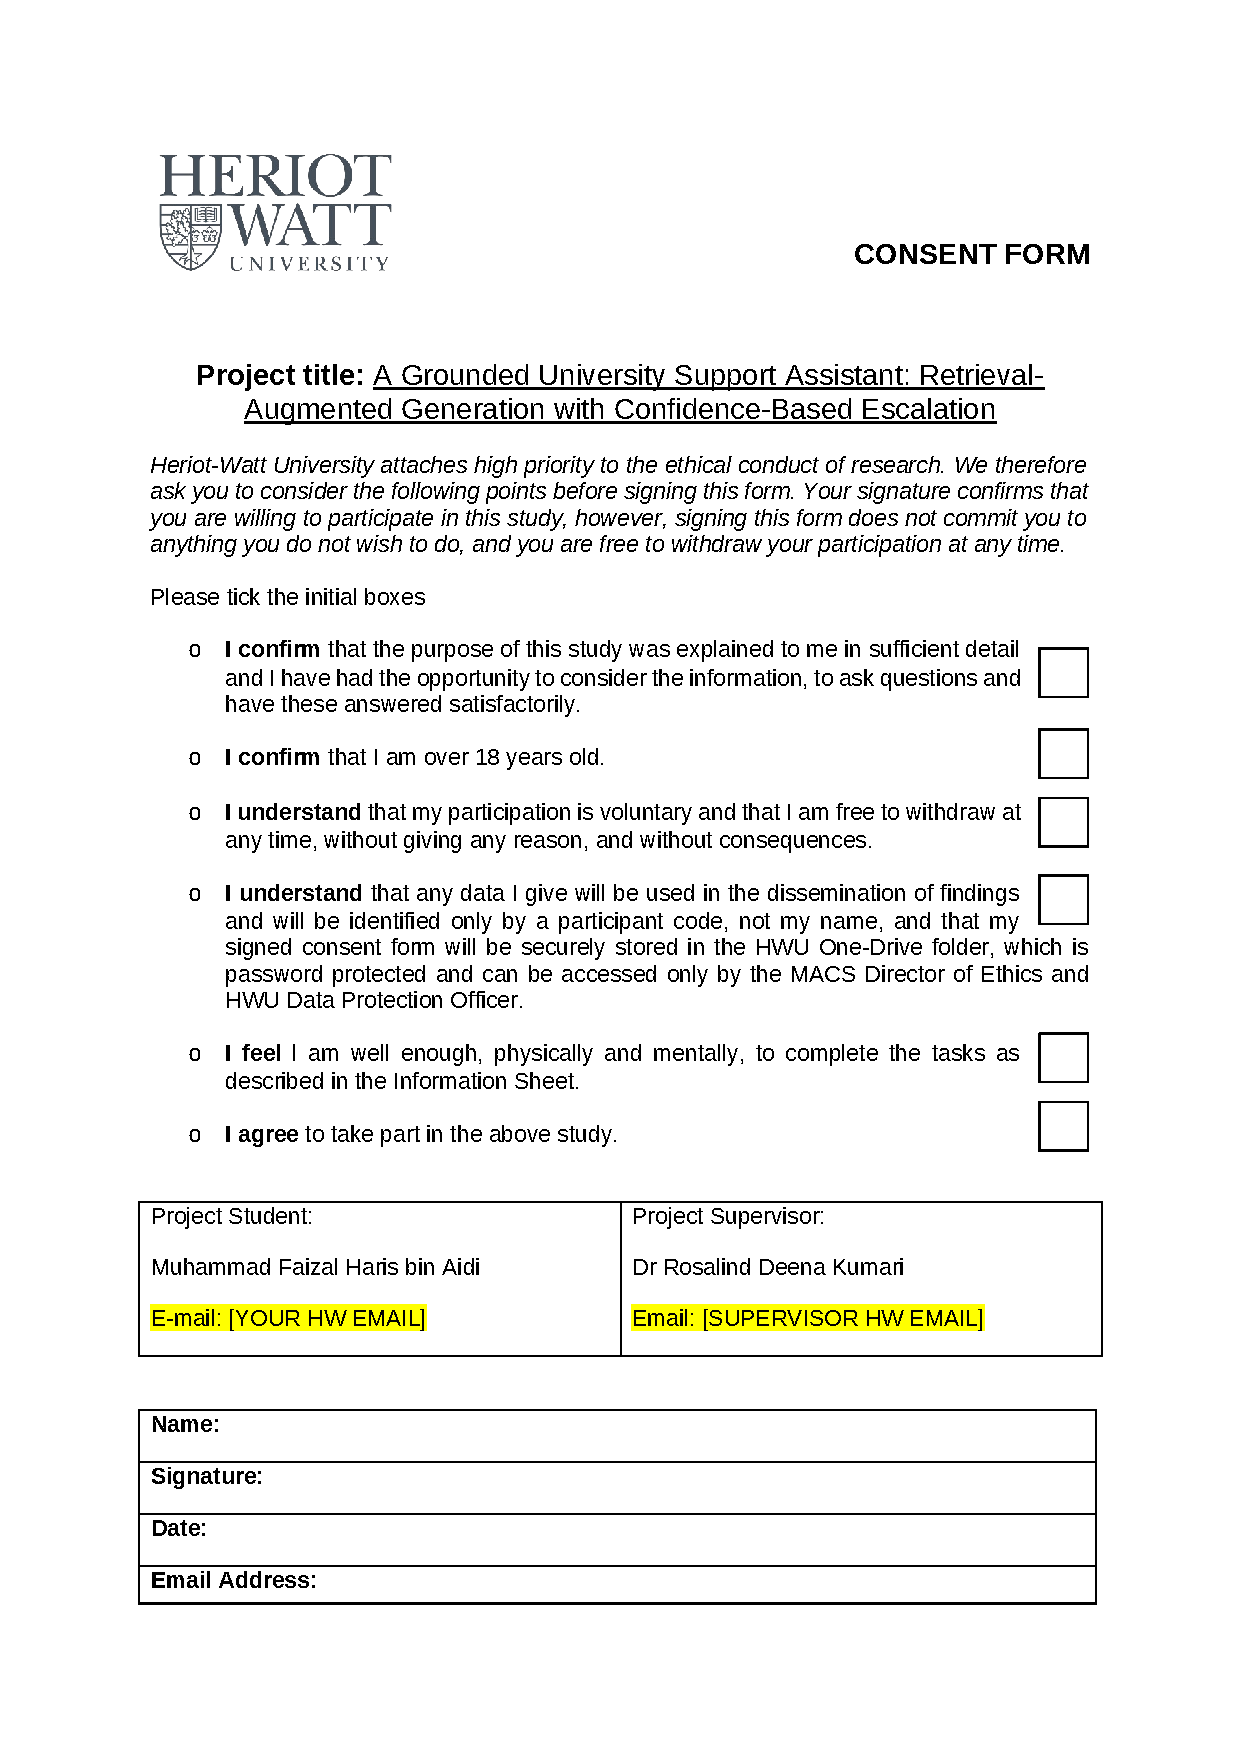
\includepdf[pages=-, scale=0.8, frame, pagecommand={}]{images/appendix_consent_form.pdf}

\section{Research Participant Questionnaire} \label{sec:app_questionnaire}

The questionnaire (prepared questions, System Usability Scale \cite{brooke1996sus} and trust items) was submitted with the ethics application, approved in November 2026, and will be used in E4.

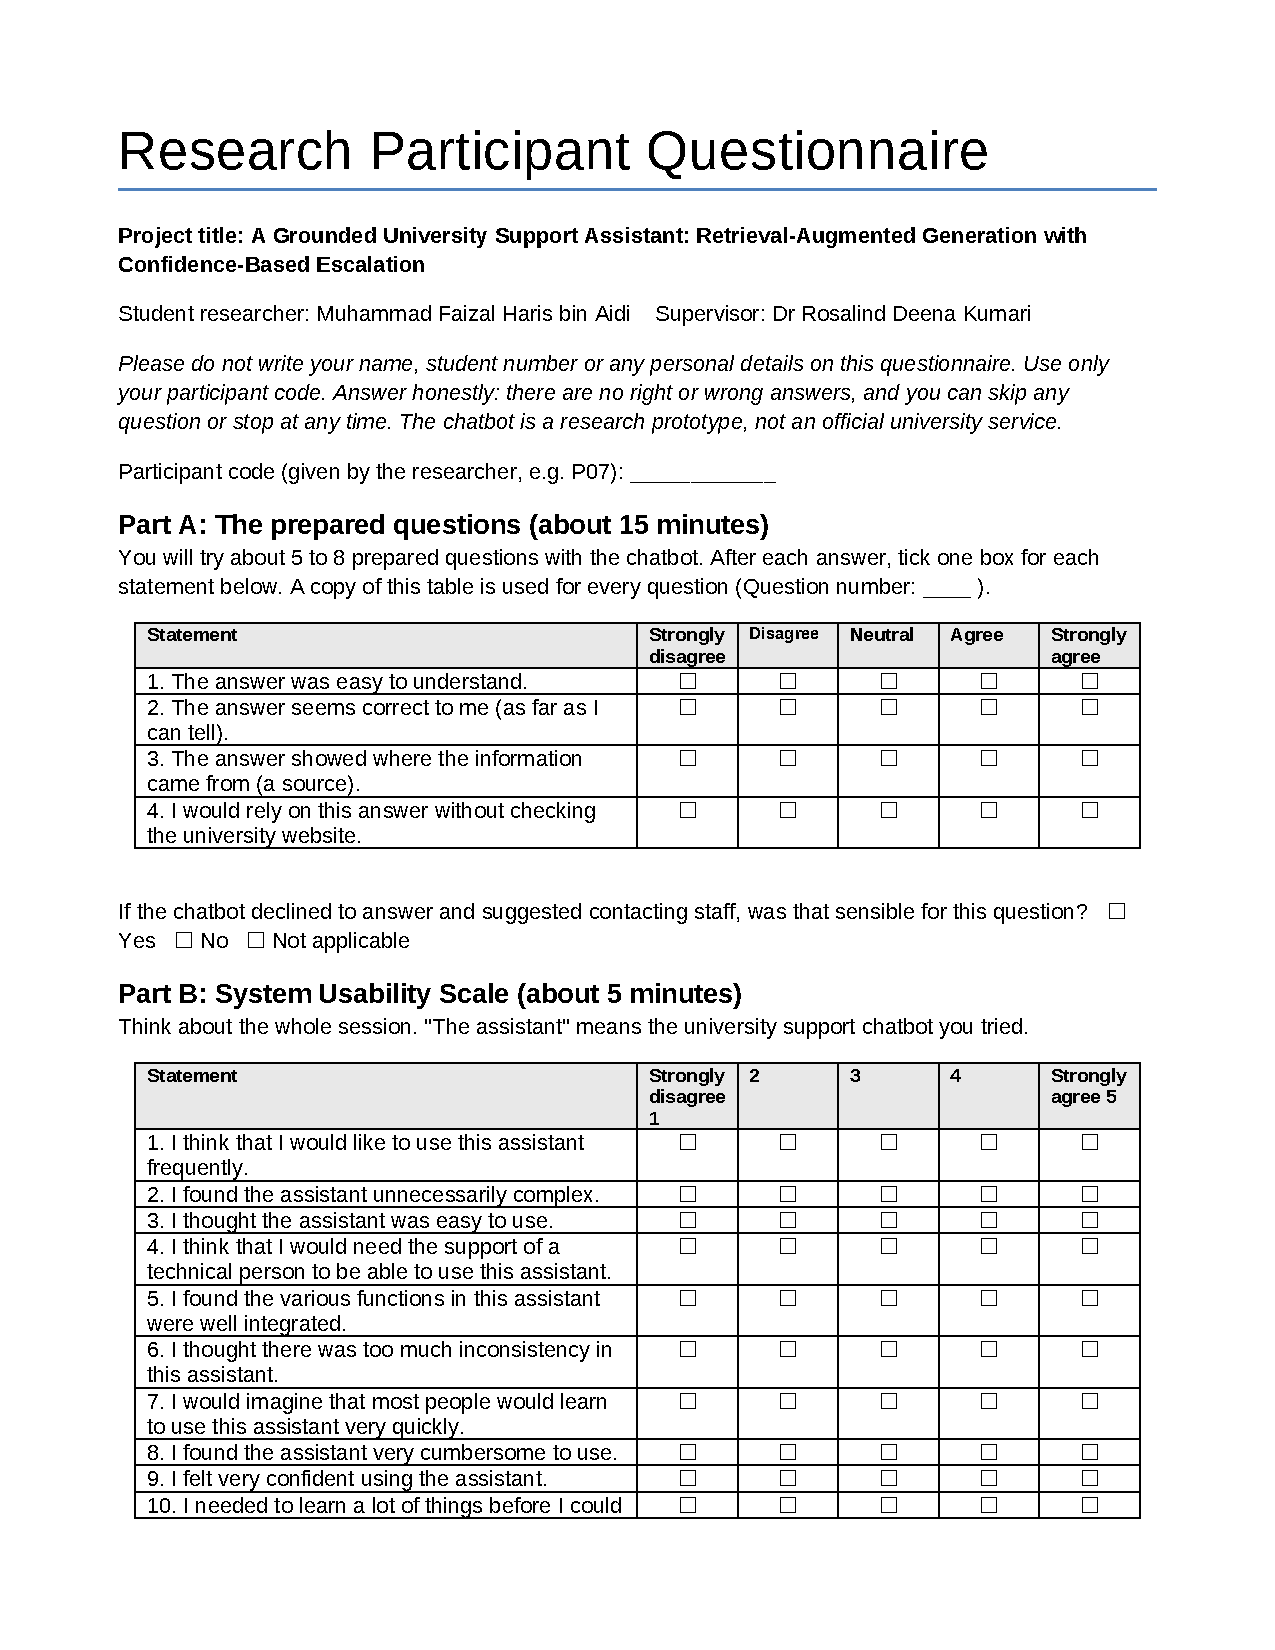
\includepdf[pages=-, scale=0.8, frame, pagecommand={}]{images/appendix_questionnaire.pdf}


% Rest of appendices...

\end{document}
